% Copyright (C) 2014-2017 by Thomas Auzinger <thomas@auzinger.name>

\documentclass[draft,final]{vutinfth} % Remove option 'final' to obtain debug information.

% Load packages to allow in- and output of non-ASCII characters.
\usepackage{lmodern}        % Use an extension of the original Computer Modern font to minimize the use of bitmapped letters.
\usepackage[T1]{fontenc}    % Determines font encoding of the output. Font packages have to be included before this line.
\usepackage[utf8]{inputenc} % Determines encoding of the input. All input files have to use UTF8 encoding.

% Extended LaTeX functionality is enables by including packages with \usepackage{...}.
\usepackage{amsmath}    % Extended typesetting of mathematical expression.
\usepackage{amssymb}    % Provides a multitude of mathematical symbols.
\usepackage{mathtools}  % Further extensions of mathematical typesetting.
\usepackage{microtype}  % Small-scale typographic enhancements.
\usepackage[inline]{enumitem} % User control over the layout of lists (itemize, enumerate, description).
\usepackage{multirow}   % Allows table elements to span several rows.
\usepackage{booktabs}   % Improves the typesettings of tables.
\usepackage{subcaption} % Allows the use of subfigures and enables their referencing.
\usepackage[ruled,linesnumbered,algochapter]{algorithm2e} % Enables the writing of pseudo code.
\usepackage[usenames,dvipsnames,table]{xcolor} % Allows the definition and use of colors. This package has to be included before tikz.
\usepackage{nag}       % Issues warnings when best practices in writing LaTeX documents are violated.
\usepackage{todonotes} % Provides tooltip-like todo notes.
\usepackage{hyperref}  % Enables cross linking in the electronic document version. This package has to be included second to last.
\usepackage[acronym,toc]{glossaries} % Enables the generation of glossaries and lists fo acronyms. This package has to be included last.

\usepackage{listings}
\lstset{
	language=bash,
	basicstyle=\footnotesize, 
	breakatwhitespace=false
}

% Define convenience functions to use the author name and the thesis title in the PDF document properties.
\newcommand{\authorname}{Bernhard Gößwein} % The author name without titles.
\newcommand{\thesistitle}{Designing a Framework gaining Repeatability for the OpenEO platform} % The title of the thesis. The English version should be used, if it exists.

% Set PDF document properties
\hypersetup{
    pdfpagelayout   = TwoPageRight,           % How the document is shown in PDF viewers (optional).
    linkbordercolor = {Melon},                % The color of the borders of boxes around crosslinks (optional).
    pdfauthor       = {\authorname},          % The author's name in the document properties (optional).
    pdftitle        = {\thesistitle},         % The document's title in the document properties (optional).
    pdfsubject      = {Subject},              % The document's subject in the document properties (optional).
    pdfkeywords     = {a, list, of, keywords} % The document's keywords in the document properties (optional).
}

\setpnumwidth{2.5em}        % Avoid overfull hboxes in the table of contents (see memoir manual).
\setsecnumdepth{subsection} % Enumerate subsections.

\nonzeroparskip             % Create space between paragraphs (optional).
\setlength{\parindent}{0pt} % Remove paragraph identation (optional).

\makeindex      % Use an optional index.
\makeglossaries % Use an optional glossary.
%\glstocfalse   % Remove the glossaries from the table of contents.

% Set persons with 4 arguments:
%  {title before name}{name}{title after name}{gender}
%  where both titles are optional (i.e. can be given as empty brackets {}).
\setauthor{}{\authorname}{}{male}
\setadvisor{Ao.Univ.Prof. Dipl.-Ing. Dr.techn.}{Andreas Rauber}{}{male}

% For bachelor and master theses:
%\setfirstassistant{Ao.Univ.Prof. Dipl.-Ing. Dr.techn.}{Andreas Rauber}{}{male}
\setfirstassistant{Dr.}{Tomasz Miksa}{}{male}
%\setthirdassistant{Pretitle}{Forename Surname}{Posttitle}{male}

% For dissertations:
%\setfirstreviewer{Pretitle}{Forename Surname}{Posttitle}{male}
%\setsecondreviewer{Pretitle}{Forename Surname}{Posttitle}{male}

% For dissertations at the PhD School and optionally for dissertations:
%\setsecondadvisor{Pretitle}{Forename Surname}{Posttitle}{male} % Comment to remove.

% Required data.
\setaddress{Vorderer Ödhof 1, 3062 Kirchstetten}
\setregnumber{01026884}
\setdate{01}{01}{2001} % Set date with 3 arguments: {day}{month}{year}.
\settitle{\thesistitle}{Entwurf eines Frameworks zur Unterstützung von Reproduzierbarkeit für die OpenEO Plattform} % Sets English and German version of the title (both can be English or German). If your title contains commas, enclose it with additional curvy brackets (i.e., {{your title}}) or define it as a macro as done with \thesistitle.
\setsubtitle{}{} % Sets English and German version of the subtitle (both can be English or German).

% Select the thesis type: bachelor / master / doctor / phd-school.
% Bachelor:
%\setthesis{bachelor}
%
% Master:
\setthesis{master}
\setmasterdegree{dipl.} % dipl. / rer.nat. / rer.soc.oec. / master
%
% Doctor:
%\setthesis{doctor}
%\setdoctordegree{rer.soc.oec.}% rer.nat. / techn. / rer.soc.oec.
%
% Doctor at the PhD School
%\setthesis{phd-school} % Deactivate non-English title pages (see below)

% For bachelor and master:
\setcurriculum{Software Engineering and Internet Computing}{Software Engineering and Internet Computing} % Sets the English and German name of the curriculum.

% For dissertations at the PhD School:
%\setfirstreviewerdata{Affiliation, Country}
%\setsecondreviewerdata{Affiliation, Country}


\begin{document}

\frontmatter % Switches to roman numbering.
% The structure of the thesis has to conform to
%  http://www.informatik.tuwien.ac.at/dekanat

\addtitlepage{naustrian} % German title page (not for dissertations at the PhD School).
\addtitlepage{english} % English title page.
\addstatementpage

\begin{danksagung*}
\todo{Ihr Text hier.}
\end{danksagung*}

\begin{acknowledgements*}
\todo{Enter your text here.}
\end{acknowledgements*}

\begin{kurzfassung}
\todo{Ihr Text hier.}
\end{kurzfassung}

\begin{abstract}
\todo{Enter your text here.}
\end{abstract}

% Select the language of the thesis, e.g., english or naustrian.
\selectlanguage{english}

% Add a table of contents (toc).
\tableofcontents % Starred version, i.e., \tableofcontents*, removes the self-entry.

% Switch to arabic numbering and start the enumeration of chapters in the table of content.
\mainmatter

\chapter{Introduction}\label{Introduction}
\section{Motivation}\label{Motivation}
Over the last decades remote sensing agencies have increased the variations of data processing and therefore the amount of resulting data. To preserve the data for further usage in the future it is necessary to have citable data and processes on the data to ensure repeatability in a long-term.\cite{6352411} Reproducibility is discussed in many science areas such as computer science, biology and also in computational geoscience. According to \cite{Ostermann2017AdvancingSW} where the reproducibility and replicability of scientific papers in geoscience got tested, only half of the publications were replicable and none of them reproducible. In \cite{Thestateofreproducibility} a survey of geoscientific readers and authors of papers got executed, with the goal of finding reasons for the lack of reproducibility in earth observation sciences. One of the results is that even though 49\% of the participants responded that their publications are reproducible, only 12\% of them have linked the used code. The understanding of open reproducible research is different among the participating scientists, so the interpretation was more related to repeatability and replicability. The main reasons for the lack of reproducibility in computational geoscience are insufficiently method descriptions, persistence of data identifier, legal concerns, the general impression that it is not necessary and also too time consuming. 
The reproduction of other papers failed by the different individual interpretations and different software versions that produce unequal results. The main amount of issues on reproducing results were issues that required changing the code or required a deeper understanding of the procedures. Also a view system dependent issues occurred related to the usage of random access memory and installation libraries of the operating system. \cite{Thestateofreproducibility}

\section{Problem Description}\label{Problem}
Already most of the the data used in earth observation sciences are retrieved or provided via Service Oriented Architecture (SOA) interfaces. Provider like Google Earth Engine and EODC provide an Web API for retrieving and processing data. Due to a different range of functionality and a difference between the endpoints of the providers it is hard to create a workflow for more than one provider. The OpenEO project has the goal to be an abstraction layer above different EO data providers. The underlying structure consists of three parts:

\begin{itemize}
	\item Client Module: Is written in the program language of the user and transfers the users commands to the backends.
	\item Core Module: A standard on how the communication should take place between client and backend.
	\item Backend Module: The provider of the data and the services, which gets the instructions from the clients and returns the results.
\end{itemize}   
Further information on the software architecture of the project is defined in the project proposal (\cite{openeo}). Until now there is no consideration of repeatability verification of workflows for users in the OpenEO architecture.Generalised layers have the opportunity to be implemented in a way that makes processes and data scientifically verifiable and reproducible, because it handles data and processes on the data in a standardised way on different providers. Even though the range of functionality and the API endpoints are well defined in the OpenEO coreAPI the contributing content providers (OpenEO backends) will have different underlying software types and versions. The underlying technology of an OpenEO backend will also change over time and can lead to different results on the same workflow executions. Consider the following: A scientist runs an experiment using OpenEO as his research tool and gets results. The same scientist runs the same experiment with the same input some months later and gets slightly different results.The question occurs, why are the results different? Has the used data changed, has the user accidentally submitted different code or has some underlying software inside the backend provider changed. Adding a possibility for the users of OpenEO to gain this information is an important
feature for the scientific community. The aim of this thesis is to provide a possibility for users
of OpenEO to verify and validate a job re-execution on different underlying technologies of an OpenEO backend provider.\cite{openeo}
\todo{Read through and improve above text.}

\section{Aim of the Work}\label{Aim}

The expected outcome of this thesis is to discover and develop a possible framework for providing repeatability in the OpenEO project. This enables users to re-execute workflows and validate the results, so that differences on the process or data are accessible for the users. To achieve this goal a model for repeatability within the project has to be discovered and implemented to evaluate the ability of the model. The model shall then conclude recommendations for the OpenEO project on how to improve re-execution validation for the user and how it can be achieved. Considering the problem description and the recommendations above, the following research questions can be formulated:

\begin{itemize}
	\item \textbf{How can an OpenEO job re-executed be applied like the initial execution?}
	\begin{itemize}
		\item How can the used data be identified after the initial execution?
		\item How can the used software of the initial execution be reproduced?
		\item What data has to be captured when?
		\item How can the result of a re-execution in future software versions be verified?
	\end{itemize}
	\item \textbf{How can the equality of the OpenEO job re-execution results be validated?}
	\begin{itemize}
		\item What are the validation requirements?
		\item How can the data be compared?
		\item How can changes of the OpenEO backend environment be recognised?
		\item How can differences in the environment between the executions be discovered?
	\end{itemize}
\end{itemize}

\section{Use Cases}\label{Use Cases}
\subsection{Capturing the Back-end environment}\label{UseCase1}
\begin{figure}[h]
	\centering
	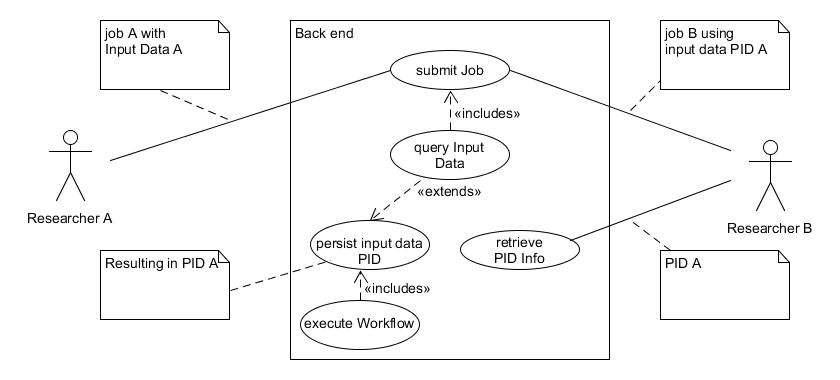
\includegraphics[width=\textwidth]{usecase1}
	\caption{Overview of the first Use Case}
	\label{fig:usecase1} % \label has to be placed AFTER \caption (or \subcaption) to produce correct cross-references.
\end{figure}
In order to make a job execution in the OpenEO project reproducible, the environment of the back end has to be captured and persisted. It has to be specified in detail and should only contain job independent information about the back end like the used operating system, programming language or used OpenEO API version. The process of capturing has to be applied automatically on each change of the back end environment. To keep track of the changes of the server and the current status, a back end version shall be introduced, which has to be updated for every change made on the back end. The point of this use case is to add the possibility to the back end provider to get automatically captured and persisted provenance data about the back end. 
The above section was describing the use case from the providers perspective and the other part is from the users perspective. It should give the user the possibility to receive information about the back ends current state. Here only data have to be shown that are not a security threat to the back end provider, but are relevant to the user. This can help the users to understand if something changed on server site. An overview of the architecture of the use case can be viewed in figure \ref{fig:usecase1}.
\subsection{Capturing job dependent environments}\label{UseCase2}
\begin{figure}[h]
	\centering
	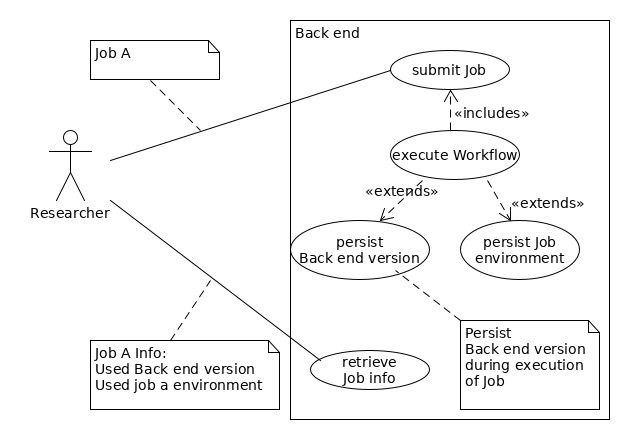
\includegraphics[width=\textwidth]{usecase2}
	\caption{Overview of the second Use Case}
	\label{fig:usecase2} % \label has to be placed AFTER \caption (or \subcaption) to produce correct cross-references.
\end{figure}
This use case is like the first one, but is only about job dependent environment information. The back end provider shall automatically get provenance data about the job execution, like used software packages and their versions. For the user additional information on a job execution has to be introduced. Calling the job endpoint, shall result in additional information interesting to the typical EO user e.g. the used GDAL\footnote{https://www.gdal.org} version. So other than the back end provider, who gets automatically all provenance data, the users only get filtered and for them relevant provenance data. The motivation for this is to add transparency of the job processing for the users, so that researchers can describe their processes in more detail. It can also help OpenEO users to understand why results differ from executions in the past. An overview of the architecture of the use case can be viewed in figure \ref{fig:usecase2}. 
\subsection{Getting differences of job executions}\label{UseCase3}
\begin{figure}[h]
	\centering
	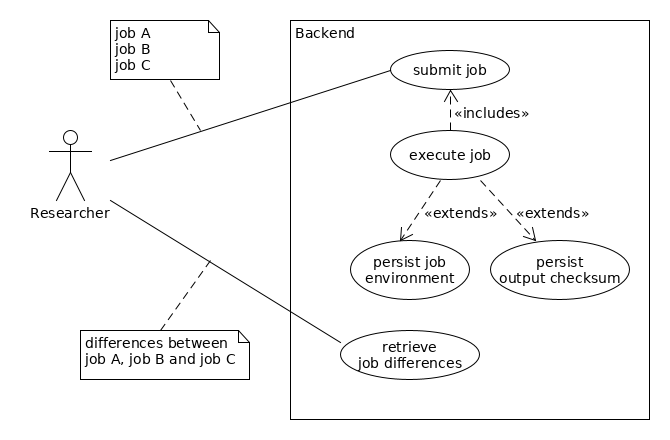
\includegraphics[width=\textwidth]{usecase3}
	\caption{Overview of the third Use Case}
	\label{fig:usecase3} % \label has to be placed AFTER \caption (or \subcaption) to produce correct cross-references.
\end{figure}
The third use case is dedicated to the OpenEO users. The goal is to add a possibility for users of OpenEO to compare different jobs not only by their results, but also on the way they were executed. The comparison is between a job execution and another job executions on the same back end. Therefore, the processing and the input data has to be identifiable. To make the comparison interesting to the users there also has to be additional information. For usability the comparison needs to be easy to apply and therefore accessible in the environment of the user, so the OpenEO client. In addition to the previous conditions a visualization of the differences for the users can lower the access barrier for users to use the feature. An overview of the architecture of the use case can be viewed in figure \ref{fig:usecase3}.

\section{Methodological Approach}\label{Method}
The use cases defined in the previous section require specific changes to the back end. In the following list the parts of the suggested solution are briefly described. 


\begin{enumerate}
	\item \textbf{Data Identification}
	In order to accomplish the capturing of processing workflows described in the use cases in section \ref{Use Cases}, the input data has to be identifiable. In order to achieve this the recommendations of the RDA (see \cite{Rauber2016IdentificationOR}) have to be implemented by additional versioning and query databases. 
	
	\item \textbf{Process Versioning}
	To accomplish the verification of different process executions, the process has to be identifiable. Therefore, a versioning of the process code can be used to persist different states of the code. The thesis is for an OpenSource project and the code of the back ends are published at Github, so Git is used as the tool to capture the code state. 
	
	\item \textbf{Additional Information}
	In order to gain a interesting description for users of OpenEO some additional information about the data and the code has to be persisted. This information is forwarded to the user at the job verification use case.   
	
	\item \textbf{User Endpoints}
	The interface for the user has to be implemented so that the use cases can be executed by the users. Therefore, the OpenEO client and core API has to be modified. The client modified in this thesis is the python client. 
\end{enumerate}

\section{Structure of Work}\label{Structure}
The following sections are structured as follows:
Chapter 2 gives an overview of related scientific activities in the area of reproducibility in the earth observation sciences and reproducibility in other areas with similar objectives.
Chapter 3  describes the technologies and concepts that are used in the implementation of this thesis. This chapter also provides an overview of the EODC back end used for the implementation
Chapter 4 provides the concept to address the research questions defined in section \ref{Aim}.  This is the theoretical definition of what has to be implemented in the OpenEO project.
Chapter 5 has a detailed explanation to the proof of concept prototype implementation and how the concept of chapter 4 was realized for the EODC back end. 
Chapter 6 dives into the evaluation of the implementation by applying the use cases to the implementation of chapter 5.
Chapter 7 summarizes the outcome of the implementation and evaluation. It contains a discussion about possible flaws and future work. 

\chapter{Related Work}\label{Related Work}


\section{Reproducibility}\label{Reproducibility}
According to \cite{6064509} reproducibility is defined as the re-run of an experiment by a different researcher in the manner of the original experiment. Repetition on the other hand is the re-run of the exact same experiment with the same method, same environment and very similar result. 
Reproducibility is a common problem in all scientific areas. It is an issue of the whole scientific community to produce results that are reproducible. Therefore in \cite{10.1371/journal.pcbi.1003285} there are ten rules defined to gain a common sense about reproducibility in all science areas. They consist of the basic idea that every result of interest has to be associated with a process and data of how it was produced. External programs have to be persisted as well as custom script versions. So the usage of version control is recommended. There is also a rule to make the scripts and the results publicly available. \cite{10.1371/journal.pcbi.1003285} 
Reproducibility is also the key element of The Fourth Paradigm \cite{noauthororeditorfourth} which is leads to the term eScience, which has the aim of bringing science and computer technologies closer together. The basic idea is to enable science in the new information technologies with data intensive sciences. The expected result of eScience is to get all scientific papers publicly available including the necessary data and processes so that scientists are able to interoperate with each other. \cite{noauthororeditorfourth}
The eScience has the potential to enable a boost in scientific discovery by providing approaches to make digital data and workflows citable. In \cite{Rauber2015RepeatabilityAR} is a common way of reaching this goal formulated. It describes an approach to look at whole research processes, other than only data citation by introducing Process Management Plans. The capturing, verification and validation of the needed data for a computational process is also demonstrated within the paper.\cite{Rauber2015RepeatabilityAR}
The main problem of computer sciences is that a lot of published papers are not provided by enough information so that they are reproducible. The problem will not be solved by the scientists that need to do additional afford to make reproducibility possible, but by providing new tools for scientists that do it for them automatically as stated in \cite{MIKSA201725}. One major problem is that the used software technologies are deprecated and not available any more, so the context of the execution has to be persisted to make a re-execution of the experiment possible. One proposed concept of doing so is the VFramwork described in \cite{Miksa2013FrameworkFV}. 

\begin{figure}[h]
	\centering
	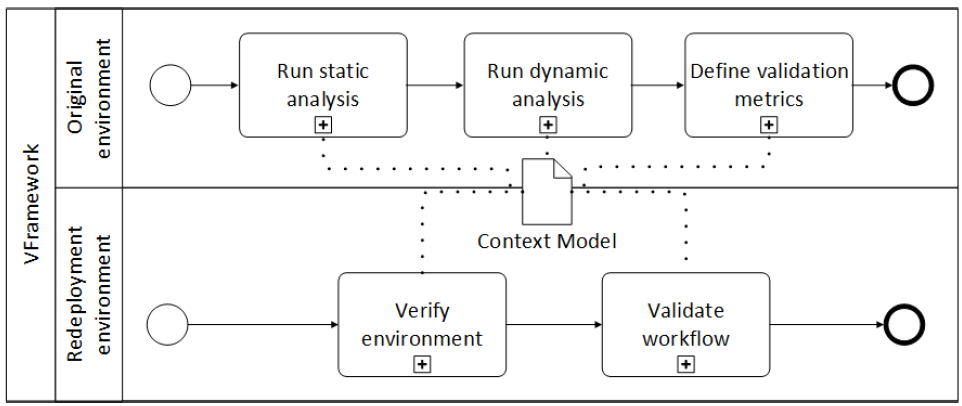
\includegraphics[width=\textwidth]{vframework}
	\caption{Overview of the Concept of the VFramework \cite{Miksa2013FrameworkFV}}
	\label{fig:vframework} % \label has to be placed AFTER \caption (or \subcaption) to produce correct cross-references.
\end{figure}

The basic concept of the VFramework is that the execution is done with parallel capturing of provenance data that is divided into the static and the dynamic data. All of which is persisted in the context model of the execution. A re-execution can then be verified and validated using the provided provenance data in the context model of the original execution and the context model of the re-execution.\cite{Miksa2013FrameworkFV}
\todo{Move VFramework to Methology and explain it in more detail}
Data citation is a key issue of reproducing results of past experiments, because they are the backbone of the execution. If the data used in an experiment is not available anymore, or not specified explicit enough then there is no chance of reproducing it no matter how much information about the execution was persisted. 
That is why there is an official working group named Working Group on Data Citation (WGDC) created 14 recommendations on data citation further explained in section \ref{Data Identification}.

\section{Earth Observation Science}\label{EOScience}

Reproducibility is a well discussed issue of the computational geoscience. The big data of earth observation science leads to complex research programs and therefore a lot of complexity in the papers.  According to \cite{Ostermann2017AdvancingSW} where the reproducibility and replicability of scientific papers in geoscience got tested, only half of the publications were replicable and none of them reproducible. Nevertheless there are publications to address this lack of reproducibility in the earth observation science. 

\subsection{Vadose Zone Journal (VZJ)}\label{VZJ}
To design solutions to the lack of reproducibility the VZJ started a Reproducibility Research (RR) program in 2015. \cite{doi:10.2136/vzj2015.06.0088}
The earth observation science is a big part of VZJ publications and most of them are not conform with the open computational science guidelines. The main reasons are behaviors of scientists that do not see the overall benefit of putting effort into documentation. Therefore the VZJ started the RR program to publish alongside the scientific paper also the code and data used by the scientists for he publication, to make it easy for the scientists to publish their research work. The aim of the project is to create a community of researchers with a common sense of reproducibility and data citation on the platform and to animate other scientists to join the approach. \cite{doi:10.2136/vzj2015.06.0088}

\subsection{The Geoscience Paper of the Future (GPF)}\label{GPF}
The geoscience paper of the future is according to \cite{Gil2016TowardTG} a proposed standard to help geoscientists to make reproducible publications. The gain of is is applying concepts of open science and reproducibility to geoscientific papers. A GPF needs to apply the following requirements:

\begin{itemize}
	\item \textbf{Reusable data} in a public repositories and persistent identifiers.
	\item \textbf{Reusable software} (including software for preparing and post editing of the data) in a  public repositories and persistent identifiers.
	\item \textbf{Documenting the computational provenance of results} in a public repositories and persistent identifiers.  
\end{itemize}

\begin{figure}[h]
	\centering
	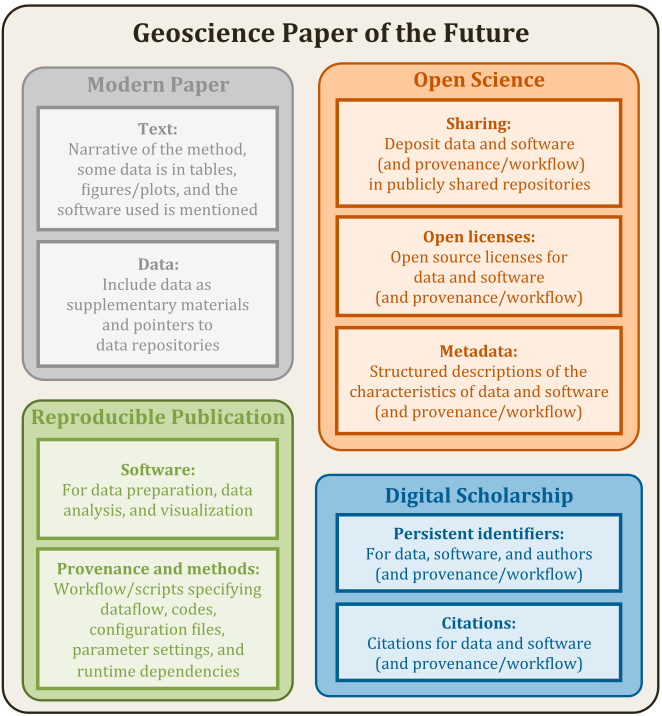
\includegraphics[width=\textwidth]{gpf}
	\caption{Comparison between reproducible publications and geoscientific papers of the future \cite{Gil2016TowardTG}}
	\label{fig:gpf} % \label has to be placed AFTER \caption (or \subcaption) to produce correct cross-references.
\end{figure}

In figure \ref{fig:gpf} the differences with a reproducible paper gets visualised. In addition to the characteristics of the reproducible paper the GPF focuses on publishing the data publicly with open licences including citable persistent identifiers.
The GPF consists of a set of 20 recommendations for geoscientists regarding data accessibility, software accessibility and also provenance information. 


\section{OpenEO}\label{OpenEO}
The OpenEO project contains of three modules, the client modules written in the programming language of the users, the back end drivers that makes it possible for every backend to understand the calls from the clients and the core API that specifies how the communication should take place. So the core API is a standard that the back end providers accepted to implement on their systems. The back end drivers are the translation of the client calls to the back end specific API. This architecture decouples the clients from the back ends so that every client can connect to every back end that applies to the OpenEO core API standard see figure \ref{fig:api2} \cite{openeo}.   

\begin{figure}[h]
	\centering
	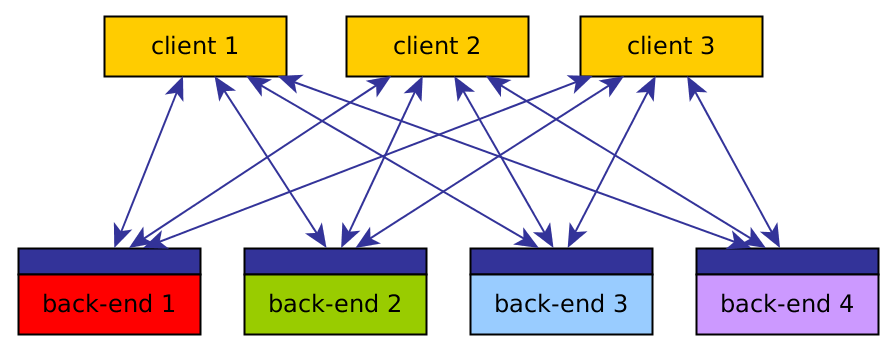
\includegraphics[width=\textwidth]{api2}
	\caption{Overview of the OpenEO architecture. \cite{openeo}}
	\label{fig:api2} % \label has to be placed AFTER \caption (or \subcaption) to produce correct cross-references.
\end{figure}


The communication is specified as an OpenAPI description and consists of all RESTful services that can be called at the back ends. Most of the calls are only to receive information about the processes and the data of the specific back end, but there are also endpoints to apply job executions specified by the user. In this thesis the focus lies on the job execution, because this is the core feature of the OpenEO project and needs to be reproducible. In the next chapter the job execution process is described in more detail. \cite{openeo}
\todo{Explain RESTful and OpenAPI a little bit ... (GET, POST, PUT usw..) -> see new Literature on Google Drive}
\todo{Explain JSON a little bit -> see new Literature on Google Drive}

\subsection{Job Execution}\label{Job Execution}
The job execution workflow in OpenEO starts at a client application that let the user define what has to be processed in the specific programming language.
The main part of the job execution is based on the description of what the back end needs to do with what data. Therefore OpenEO introduces the process graph, which consists of a tree structure describing the processes with their data and the input data identifier, which is back end specific. The process graph is in a JSON format and gets generated by the clients in the background without the users seeing it directly. In figure \ref{fig:process_graph} there is an example of a process graph. 

\begin{figure}[h]
	\centering
	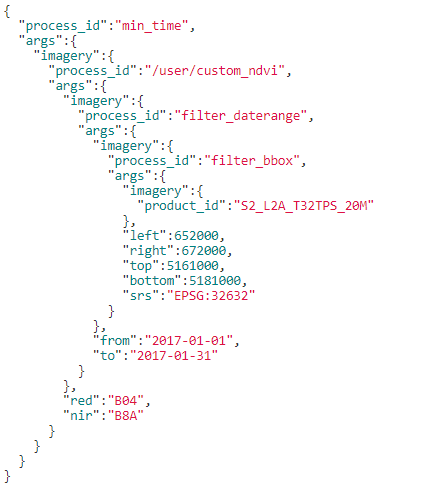
\includegraphics[width=\textwidth]{process_graph}
	\caption{Proof of Concept process graph of the EODC back end for the OpenEO core API version 0.0.2 . \cite{openeo}}
	\label{fig:process_graph} % \label has to be placed AFTER \caption (or \subcaption) to produce correct cross-references.
\end{figure}

The back ends interpret the process graph from inside out. Inside figure \ref{fig:process_graph} the element in the middle defines the input data identifier in the \"imagery\" block, with the \"product\_id\". In this case the \"s2a\_prd\_msil1c\" is the chosen input data identifier. Now the back end goes one step up in the hierarchy of the process graph and calls the process \"filter\_bbox\" with the parameters \"left\", \"right\" and so on using the input data. The output data of the previous process is also the input data of the next process. It is possible that the input of a process is a whole new process graph. In figure \ref{fig:process_graph_diagram} the same process graph is visualized from the back end point of view, so how it gets interpreted. 

\begin{figure}[h]
	\centering
	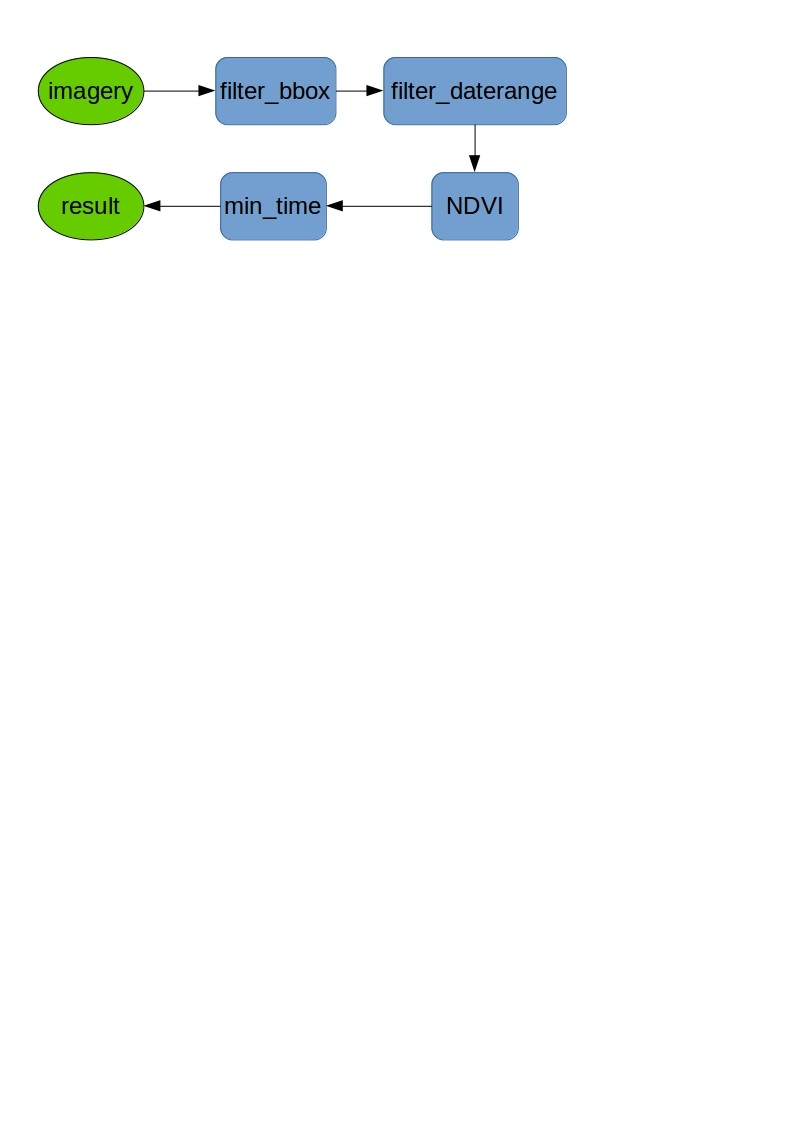
\includegraphics[width=\textwidth]{process_graph_diagram}
	\caption{TODO figure number combine the two figures? -> maybe use official ones ...}
	\label{fig:process_graph_diagram} % \label has to be placed AFTER \caption (or \subcaption) to produce correct cross-references.
\end{figure}

There are two different kinds of process executions depending on the back ends capabilities, synchronous and asynchronous calls. Synchronous calls are directly executed after they got received from the back end and the user that sends the process graph has to wait until the job is finished. For example on the python client the program waits after sending the process graph to the back end until the back end returns the result and the results are directly returned to the user. On the asynchronous call the user sends the process graph, but it does not get executed until the user starts the execution on the back end through an additional endpoint. When the processing is finished the user can download the result at another endpoint of the back end. For the asynchronous calls there is also the possibility to subscribe to a notification system on the backend, so that the user gets notified when the job execution finishes.     
The processes are defined at the OpenEO core API and therefore independent from the back end they get called, other than the data identifier, which is different for every back end.  
\\
The previous example shows a process graph that only uses predefined processes and data. Within the OpenEO project there is the possibility to define individual processes and execute them on the back end. In the project they are called “user defined functions” and are at the writing of this thesis not well defined, but are basically code written by the OpenEO user that gets sent to the back end and executed at a secure environment. The user can define processes and can run them with the data provided at the back end, using the infrastructure of the back end. Every back end has to individually define what the restrictions on user defined functions are. 
There is also the possibility to upload files to the back end that can be used within the process graph. The user can upload the file through an explicit endpoint of the back end. After the upload finished, the file can be referenced inside the process graph.\todo{[TODO: Quelle Github Docu Release Version 0.0.2]}

\subsection{Back end Overview}\label{Back end Overview}
Even though the back ends implement the OpenEO core API standard, they are still very diverse behind the abstraction layer. Some back ends has already an API, where the OpenEO calls have to be adapted to. There are 7 partners within the OpenEO project that are implementing a back end driver. The back ends have to manage the translation of the process graph to the actual code that executes the defined process chain. Also the billing of the users is completely different on every back end. 
\todo{Create overview of the different Back ends of the project}

\section{Existing Tools}\label{Existing Tools}
In this section tools that are designed to solve similar problems like this thesis get summarized and described further. There is also an explanation why the specific tool was not used for the purpose of this thesis. 

\subsection{ReproZip}\label{ReproZip}
ReproZip is a packaging tool to enable the reproducibility of computational executions of any kind. It automatically tracks the dependencies of an experiment and saves it to a package that can be executed on another machine by ReproZip. It is even capable letting the reexecuter modify the original experiment. It was developed for the SIGMOD Reproducibility Review. In figure \ref{fig:reprozip} the architecture of ReproZip is shown in detail. It traces the system calls to create a package defined in the configuration file. So that a single file of file type “.rpz” gets produced. This can be unpacked on a different machine or by a different user and then be re-executed. The aim of the tool is to make reproducibility easy to apply for single experiments. \cite{29c5846926a4497d95f276604cb0368c} That is the reason why it is not used in the solution of this thesis, the captoring  is to fine granulated and takes too much performance from the back ends, which is a key selling point for back end providers. The payment for users of OpenEO, depending on the back end, may have to pay by the duration time of the processing. Another issue with ReproZip is that it is not possible on to capture the big data of the back ends within the package, because it would take too much space.  

\begin{figure}[h]
	\centering
	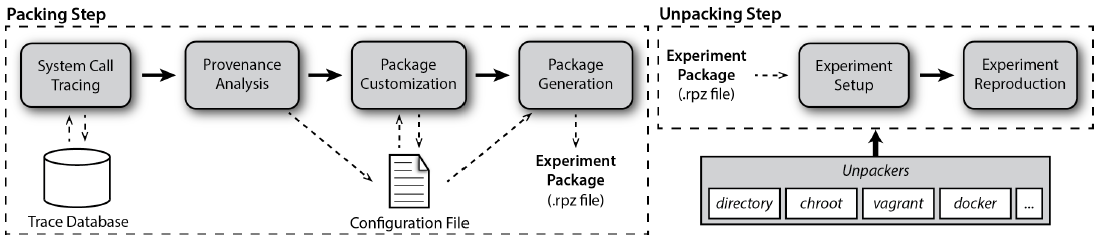
\includegraphics[width=\textwidth]{reprozip}
	\caption{TODO figure number combine the two figures? -> maybe use official ones… }
	\label{fig:reprozip} % \label has to be placed AFTER \caption (or \subcaption) to produce correct cross-references.
\end{figure}

\subsection{Docker / Smartcontainer}\label{Smartcontainer}
Docker containers are very common in geoscience executions. The advantages on reproducibility and cost savings by using docker containers is discussed in \cite{rs9030290} for the Geographic Object-Based Image Analysis (GEOBIA). The docker implementation of the image analysis was implemented with an docker image including a user interface that can be used by non-experts. There are also experiments for the more general Object-Based Image Analysis (OBIA) with docker containers presented in \cite{proceedings456}. The conclusion of the experiment is very positive with only little shortcomings in the usability. The two papers mentioned above are using the docker images to make it easy to re-run an experiment on the OBIA system, but the remaining question is how the docker configuration can be preserved in a manner so that it can be reproduced in different environments. The aim of \cite{emsley2017a} is to answer this question by introducing in addition to the Dockerfile a workflow file saving the environment and entities involved. A SPARQL query got introduced to create the possibility to use the container as a repository of metadata regarding the container. 
Another approach of preserving a docker container is smart container introduced in \cite{Huo2015SmartCA}. The aim of smart container is an ontology and software to preserve docker metadata. It uses the PROV-O standard to define the docker provenance. 
Docker containers are not part of the solution of this thesis, because the impact of the implementation shall not be too big for the back end providers, because reproducibility is not a main goal of OpenEO and the afford on implementing it on the back ends is limited. The solution has to be simpler and more general to be applied on all different back ends. Even so can docker containers be used to apply the defined context model in \ref{Design}.

\chapter{Methodology}\label{Methodology}

\section{Version Control Systems}\label{Version Control Systems}
Version control systems (VCS) became a very important part in all computational sciences. It enables to save different versions of a piece of code and the possibility to jump back to a certain version of it. Before that programmers tend to have multiple directories to version the code. The basic idea of VCS is that via a command line interface it is possible to set a version of the current state of the code. These versions can be accessed in future, without changing other versions of the code and without multiple folders. \cite{10.1109/MCSE.2009.194}
In this thesis Gitorious (Git) is used as version control system. Versions in git are defined as commits and are stored locally, but can be published to an external server, where, depending on the user rights, they are accessible for other users. So the commits are stored locally and remotely. \cite{QuickGit} In OpenEO Git is used as the versioning tool and GitHub is used as the publicly available server. Since OpenEO is an open source project, the code of every back end, core API and client is available at GitHub. In this thesis the Git commit and the GitHub repository is used as an identifier of the code running at the back end. 

\section{Hash}\label{Hash}
Hash functions are used to validate the data without having to save the whole data. They have three important properties to work properly. First it has to be difficult that two different input data has the same hash outcome. Second is should be difficult to get back to the original data from the hash information. Last but not least is has to be hard to find a message with the same hash value as a already known message. The above properties makes the hash functionality common to identify data without having to save the original one. \cite{3b412889270f46f59740fbf1ca8cd7e0} There are a lot of different hash functions available. In this thesis the SHA-256 gets used for the metadata of the context model, mostly to compare different data outcomes.

\begin{figure}[h]
	\centering
	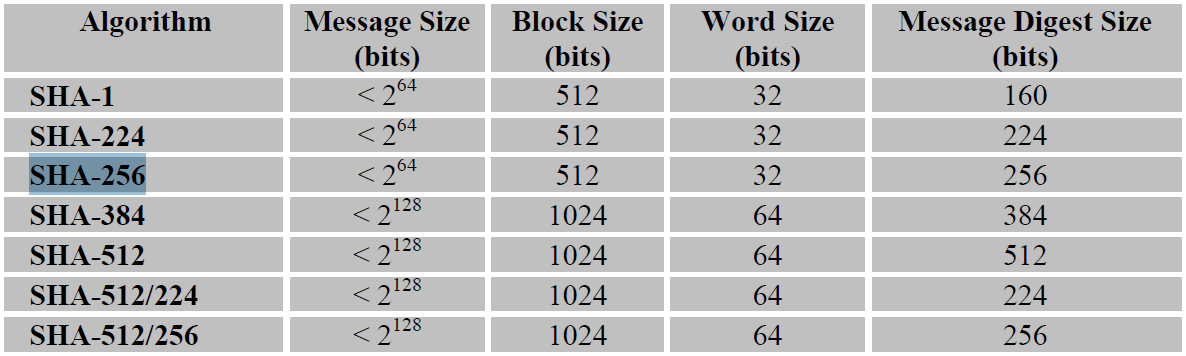
\includegraphics[width=\textwidth]{sha}
	\caption{\cite{shapaper}}
	\label{fig:sha} % \label has to be placed AFTER \caption (or \subcaption) to produce correct cross-references.
\end{figure}
The SHA-256 is chosen in the implementation, because of the best combination of performance and security of the above described properties of the hash. 

\section{Linux Tools}\label{Linux Tools}
In the solution a view linux tools are used for capturing the provenance of the back end, therefore the used tools get described in this section. 

\textbf{dpkg}
The host system was a debian based system and therefore the dpkg tool was used to get the installed packages of the system. All packages installed by the debian system are installed through this package manager. It has a command line interface to access all installed packages. This is used to get all installed packages of the system as part of the metadata of the back end host.\cite{dpkg}

\textbf{inotify}
The inotify service enables monitoring folders on the file system. It is capable of monitoring single files or whole directories.\cite{inotify} It consists of a lot of different tools to manage the change monitoring. In this thesis the inotifywait service is used. It waits for in the config file specified changes made to a specific directory. The changes in the config file that have to occur can be read, write or modify operations and much finer granulated operations on the directory. Every time an event happens to the directory, it get checked if it is one of the events defined in the inotify configuration and if so it gets written to an output file or the console. \cite{inotifywait} In this thesis it is used to capture changes made to the working directory of the back end. 

\textbf{cron}
Cron is used to call periodical jobs in a linux based system. It is accessed via the crontab tool that functions as a configuration file for the cron service. Inside of the crontab there it is possible to call a shell script periodically. Every line in the crontab is a different script that gets called by the cron service. A line in the crontab specifies the time in which the script has to be executed. Therefore the every minute, hour, day of month, month and day of week gets specified on which it shall be called. If there is a ”*” character, it will be called on every occasion of the time or date type. \cite{crontab}

\section{PROV}\label{PROV}
In 2003 the World Wide Web Consortium published the PROV model as a standard for provenance definitions.  The standard is defined by twelve different documents. In this thesis only the PROV Ontology document is used in the implementation. \cite{f06eee9045b445be89cf07100b3ce05c}
PROV Ontology (PROV-O), which is a standard language used to describe OWL2 Web Ontology. It is designed as a lightweight concept to be used in a broad spectrum of applications. 

\begin{figure}[h]
	\centering
	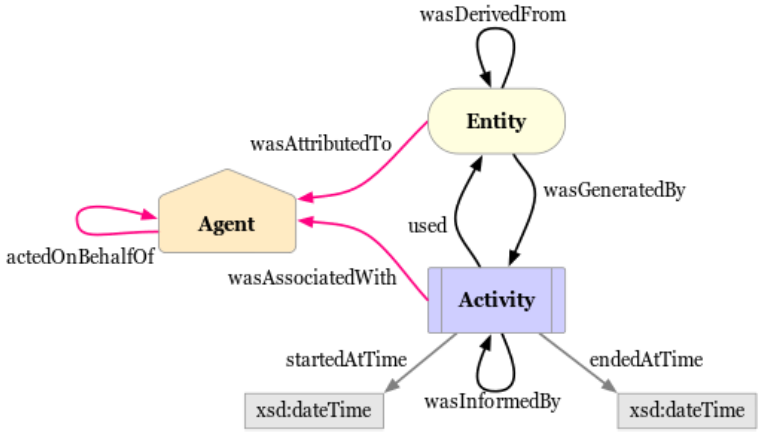
\includegraphics[width=\textwidth]{prov}
	\caption{Overview of the main components of PROV-O \cite{733f89c65e4844f9aabcae1c276a5602}}
	\label{fig:prov} % \label has to be placed AFTER \caption (or \subcaption) to produce correct cross-references.
\end{figure}

In figure \ref{fig:prov} there is the basic setup of the PROV concept. It consists of three main elements. The Entity is any physical, digital, conceptual thing. Provenance records describe entities and entities can consist of references to other entities. Another element is the Agent, which is responsible for activities and that activities are taking place. Examples for Agents are software, persons or organisations. The association of an Agent to an Activity defines the responsibility of the Agent to the Activity. An Activity describes what happened that the Entity has come to existence and how attributes of an Entity changed.\cite{f06eee9045b445be89cf07100b3ce05c} In this thesis the PROV-O standard is used by a feature of the back end to transform the context model of a process graph to an PROV-O description (see section \ref{Implementation:User Interface}). 

\section{Noworkflow}\label{Noworkflow}

In one of the process provenance capturing implementation is noworkflow used. Therefore it gets introduced in this section. Noworkflow was introduced in \cite{c9e0604becba42af96a9cb0a6f60018b} as a script provenance capturing tool with the aim to not affect the way users implement their experiments. As proof of concept the noWorkflow command line tool got implemented for python. The provenance is captured in SQLite database by different trials, which are executions of the experiment. The main benefits of noWorkflow is that it does not instrument the code and it automatically captures the definition, deployment and execution provenance in a local SQLite database. The provenance data can then be accessed via the command line interface of noWorkflow and there are also some analyses features added.\cite{c9e0604becba42af96a9cb0a6f60018b}

\begin{figure}[h]
	\centering
	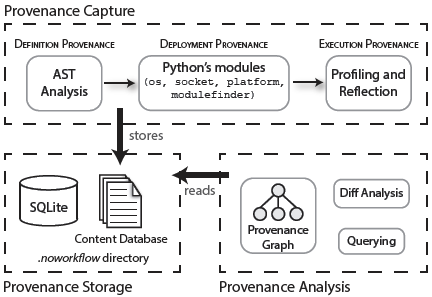
\includegraphics[width=\textwidth]{noworkflow}
	\caption{Architecture of noWorkflow \cite{c9e0604becba42af96a9cb0a6f60018b}}
	\label{fig:noworkflow} % \label has to be placed AFTER \caption (or \subcaption) to produce correct cross-references.
\end{figure}

The noWorkflow framework got improved over time so that in \cite{Pimentel2016TrackingAA} an additional feature of tracking the evolution of the experiment execution. It adds the possibility to compare different trials of an experiment and to visualize the history of past executions. In \cite{Pimentel:2016:FPC:3090188.3090214} the fine-graned provenance tracking got added to noWorkflow, so that the execution of the python script can be viewed of a set of execution lines. It also adds a visualization of all called functions with some limitations on multiple function calls in one line, dictionaries and lists. In \cite{69bac1252a684629baa43b48e350068d} the provenance capturing of noWorkflow in combination of yesWorkflow, which gatheres information about the provenance using comments and annotations (see \cite{192094}), got combined. The combination enabled a broader provenance information, querying and visualizations. 
In this thesis noworkflow is used in the first attempt of the implementation of the context model capturing described in section \ref{Implementation:Noworkflow Implementation}.

\section{Data Identification}\label{Data Identification}
Data identification and citation is a main concern in many computer relying sciences. For the aim of this work, the input data is a key element of the capturing. If the input data can not be identified correctly, the capturing of the process on it does not make sense. Therefore the identity of the data has to be guaranteed. The Research Data Alliance (RDA) presents general solutions to achieve data identifications. There are 14 recommendations defined to achieve the identification of an exact version and subset of input data. The recommendations are independent of the type of data and database.  In the following the most important recommendations for this thesis get briefly introduced.\cite{rauber2016identification}

\begin{itemize}
	\item \textbf{R1: Data Versioning} 
	Changes on a data record needs to result in new versions of the data record and the persistence of the deprecated data records. All data record versions need to be identifiable and accessible. 
	\item \textbf{R2: Timestamping} 
	All changes to the database have to be comprehensible via timestamps. So every time changes are applied to the data, there needs to be a timestamp when it happened. 
	\item \textbf{R3: Query Store Facilities} 
	There needs to be a query store implemented at the data provider to store queries including their metadata to be able to re-execute them in the future. The database has to store, according to \cite{rauber2016identification} the following things: 
	\begin{itemize}
		\item The original query as posed to the database
		\item A potentially re-written query created by the system (R4, R5)
		\item Hash of the query to detect duplicate queries (R4)
		\item Hash of the result set (R6)
		\item Query execution timestamp (R7)
		\item Persistent identier of the data source
		\item Persistent identier for the query (R8)
		\item Other metadata (e.g. author or creator information) required by the landing page (R11)
	\end{itemize}
	
\end{itemize}

 The recommendations in the context of the thesis are defined in more detail in section \ref{Design:Data Identification}. 

\section{EODC Back End}\label{EODC Back End}
 
 The EODC back end is one of the contributing back end providers of the OpenEO project. It is in general a python implemented back end that uses some virtualisation technologies for the job executions. The overlaying technology is OpenShift (using Kubernetes) \cite{openshift}, which is capable of scaling docker containers and handles the execution of them. In the docker containers the python code for the processing gets executed. The docker description files and the python code is available on GitHub\footnote{https://github.com/Open-EO/openeo-openshift-driver/tree/release-0.0.2}. In this thesis the latest version of the EODC back end provided in GitHub with the version 0.0.2 is used. In this version every process of the OpenEO process graph is represented by an own docker container and python code of the processing. The service layer of accessing the back end is build with the python library Flask. Even though EODC has a lot of already processed data, so satellite data that is already processed in a certain way, in OpenEO only the data from Sentinel 2 is proved by the time this thesis is written. So the underlying data are satellite images provided by the European Space Agency (ESA) from the raw data coming directly from the Sentinel 2 satellite. 
 \todo{Maybe add more detailed view on the Setup}
 
\chapter{Design}\label{Design}
In this chapter the design of the provenance capturing gets described. First the architecture of the OpenEO project gets described further. Especially the job execution path throughout the parts of OpenEO gets described, because it is the key element for the context capturing. Therefore the back end, where the jobs get executed get described in more detail. After that the context model gets presented. 

\todo{Image of general Design (Input data identification -> code identification (github) -> output hash}

\section{Data Identification}\label{Design:Data Identification}

\begin{itemize}
	\item \textbf{R1: Data Versioning}
	\item \textbf{R2: Timestamping}
	\item \textbf{R3: Query Store Facilities }
	\item \textbf{R4: Query Uniqueness}
	\item \textbf{R5: Stable Sorting}
	\item \textbf{R6: Result Set Verification}
	\item \textbf{R7: Query Timestamping}
	\item \textbf{R8: Query PID}
	\item \textbf{R9: Store the Query}
	\item \textbf{R10: Automated Citation Texts}
	\item \textbf{R11: Landing Page}
	\item \textbf{R12: Machine Actionability}
	\item \textbf{R13: Technology Migration}
	\item \textbf{R14: Migration Verification}
\end{itemize}
\todo{ToDo after Data Identification discussion with eodc}

\section{Context Model}\label{Design:Context Model}
In this section the concept of the provenance capturing is described. The aim of the capturing is to be easy to implement on the OpenEO back ends, but also powerful enough to make the reproduction of the workflows possible. The whole capturing process can be structured in three thematic parts.

\begin{enumerate}
	\item \textbf{Data identification} \\
	This part describes the needed implemented data identification recommendations based on the RDA guidelines (see \cite{rauber2016identification}). To make the processes theoretically reproducible the input data has to be identifiable. So different versions of the same data has to be distinctable and data needs to be persisted or specified in a way that it can be recreated. A description of all steps necessary for the OpenEO back ends can be viewed at section \ref{Design:Data Identification}.
	\item \textbf{Back end provenance} \\
	This part describes the provenance of the back end, that is not depending on a job execution. There has to be an automated process running on the process machine to capture every change that influences the execution of OpenEO jobs. A description of more detail can be viewed on section \ref{Design:Back end provenance} .     
	\item\textbf{Job dependent provenance} \\
	This part contains the provenance of a job execution. It consists of the workflow context and the data related to one specific job. This in combination of the back end provenance is the full provenance data to make an OpenEO job theoretically re-executable.   
	\item \textbf{User information} \\
	This part consists of all possibilities that provides users with information they want to know about the provenance of the back end and the provenance of the job execution. The aim is to provide users with information that makes them easier to choose between back ends. On the other hand the user shall be able to retrieve the provenance data of the job in a way that the back end has no security risks. This part is not directly part of the context model, but of the implementation on the user interface. 
\end{enumerate}

\subsection{Back end provenance}\label{Design:Back end provenance}
The scope of this part of the context model is to get the static environment of where the job execution at the back end takes place. It contains the provenance data that is independent from a job execution, so does not change regardless of how much jobs were processed. It can only change from inside of the back ends by their maintainers. In the OpenEO project there are a great variety of different back end providers with very different setups, so the challenge of this part is to make it as simple and generic as possible. The data captured in this part of the context model is not meant to be shown to the user directly, because of security issues. The following data gets suggested to be the minimal set of static provenance data that has to be captured. 

\textbf{B1: Code Identification}
Since the project is an open source project and every back end has a github repository were at least the basic setup is stored. The aim of this strategy is to get other back ends with similar settings to reuse the already working setups of the running back ends.  Therefore, at least during the project runtime, every back end provider has a github repository were the code is publically available. This information is added to the back end provenance by saving the git repository url, the used branch, the used commit and local changes to the repository.   

\textbf{B2: Used Folders}
The back end will most probably not only use the github repository for the processing, so that other folders are involved that stores config files or additional code. This information is also crucial for the job execution and therefore needs to be stored. Changes of this directory have to be detected and stored in the context model. Temporary written folders have to be excluded to the capturing to prevent detecting changes that are not important.    

\textbf{B3: OS and packages}
The operating system can also have an impact on the processing and so it has to be stored to the context model too. Not only the information about the operating system, but also the installed packages have to be stored in the context model. In a linux based system it is sufficient to store the location where the packages get installed (e.g. /etc). If the whole processing is done in a virtual container the operating system of that container shall be stored. If the whole processing is done in a docker container, the docker description file has to be saved in addition. But only if the docker container description does not change on different input process graphs, otherwise it has to be added to the “job dependent provenance”. 

\textbf{B4: Core API Version}
The back ends core API version is the version of the OpenEO core API version it is using. In the productive usage of the OpenEO project it can happen, that the versions of the clients and the back ends differ, so that the behavior might not compatible. So the back end server configuration depends on the core API version of OpenEO, hence it shall be added to the context model.

\textbf{B5: Back End Version}
The captured data described in the previous sections will result in a back end version. The back end version shall be an identifier (e.g. a number) that gets updated on every change of the backend considering the provenance data described above. 
\\
To  provide long term stability of the capturing, there shall be a tool to automatically capture the provenance data to the context model. Every change on any of the previously described context data has to be detected automatically and have to result in a new back end version. This can be done by a standalone capturing tool that does not need to have detailed insights into the back end. 


\subsection{Job dependent provenance}\label{Design:Job dependent provenance}
In this section the job dependent provenance of the context model gets described. The data captured is tied to an specific job execution, so for every job execution a new context model gets created. The structure of the capturing is using the defined process graph structure of OpenEO. The process graph is already a description of the processes that run at the back end. So sending the same process graph to the same back end again shall result in the same outcome. To assure that the process graph results in the same way of processing the processing itself gets captured. After receiving the job the back end will transform the process graph into code that actually does the processing. Figure \ref{fig:design_overview_common} shows the structure of the workflow capturing. 

\begin{figure}[h]
	\centering
	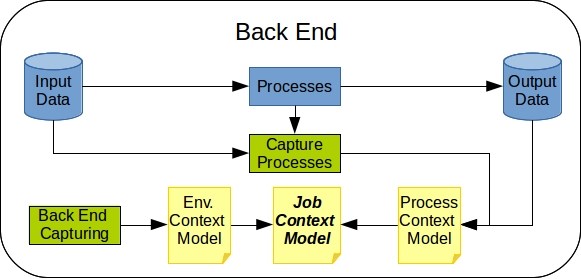
\includegraphics[width=\textwidth]{design_overview_common}
	\caption{Design Overview of capturing the job context model.}
	\label{fig:design_overview_common} % \label has to be placed AFTER \caption (or \subcaption) to produce correct cross-references.
\end{figure}

The single parts of the capturing are described more in detail in the following sections. 

\subsubsection{Input Data}\label{Design:Input Data}
The input data of the processing is crucial for the outcome of the process graph. Even though the process graph already contains an identifier for the input data that has to be unique for the specific back end, changes to this data might not result in a new identifier. So jobs called later in time might use another version of the input data than the previous jobs. To prevent this the input data has to be persisted according to the 14 steps of data provenance defined by the RDA \cite{rauber2016identification}. Every back end is responsible for applying a data version, for this context model it is assumed that the back ends preserve the data as described in \ref{Design:Data Identification}. Nevertheless, the current core API version (v0.0.2) is not capable of letting the user choose, which version of data the user want to use. Hence, there has to be an addition to the process graph so that product identifier has an additional time-stamp. So every input data identifier has now a time-stamp for when the data was retrieved. The meaning of the time-stamp is to tell the back end that the user wants to use the data at the time of the time-stamp. This gives the back ends the possibility to design their own strategy of applying a version to the data. It has to be persisted, which version of the data was available on what date and time. This leads to the following data entries that have to be captured regarding input data.

\textbf{J1:  Source Input Data Identifier}
The source data identifiers used in the process graph, so every identifier of the “product” part of the process graph, needs to be identified by a version of the input data. The query store described in section \ref{Design:Data Identification} provides the back end with an identifier (PID) that has to be used as the input data identifier in the context model.


\subsubsection{Process Data}\label{Job:Process Data}
In this section the capturing of the process itself gets described. As mentioned above the process is described at the process graph, but to be certain that the same process id results in the same code, the code has to be captured. So the code running the processing has to be captured and has to result in a signature that can be compared to other executions. An example of doing so is to hash the entire resulting code. 
The way of executing a specific process graph is not only related to the code running it, but also by the dependencies of the code. So the environment of the code and information about the code environment has to be added to the context model. If there are any docker image, where the job is running that is not independent on the process graph has to be captured. The programming language, its version and its used packages has also to be captured and added to the job context model. To every process executed also the start time and end time has to be captured as a timestamp. So this leads to the following capturing entries in the context model.

\textbf{J2: Process Code Identifier}
The executed  code for the process has to be identifiable, therefore there has to be an id of the code. The OpenEO project is an OpenSource project and the back end provider have the used code at the Github repository, so the link to the github repository with the currently checked out commit can be used as the identifier. 

\textbf{J3: Programming Language}
The programming language of the code has to be captured. Name and version used has to be captured and added to the context model.

\textbf{J4: Installed packages of programming language}
To identify the environment of the code execution, the installed packages of the programming language has to be captured and added to the context model. The version of the packages have also to be included in the context model. For example in python the installed models have to be added with their versions to the context model.

\textbf{J5: Start and End time of process execution}
On the beginning of the process execution a time-stamp shall  be created and at the end of the process execution. These timestamps have to be persisted in the context model.

\subsubsection{Output Data}\label{Job:Output Data}
The output data of the processing has to be captured as well. In the OpenEO project the results can be rather big, that is why a simple generated hash of the output result is enough in this context model. The output data does not have to be identifiable within the scope of this thesis, but just comparable with other executions. Therefore a hash of the output data is sufficient. The aim of the output data capturing is not to add the possibility to find differences between results, but to be able to see that the results are different. 

\textbf{J6: Result Hash}
The output result of the process need to be verifiable and therefore need to be persisted. An easy way to achieve this is to take a hash over the sorted output files. 

\subsubsection{Back end provenance}\label{Job:Back end provenance}
The back end provenance described in \ref{Design:Back end provenance} has to be added to the job context model. Over time the back end provenance gets updated so that every job has to keep the back end configuration at the time of the execution. There are two possible solutions to achieve this. First the  identifier of a specific version of the back end gets added to the context model. In this case the data of the back end provenance versions have to be persisted and accessible. The second solution is to put the whole back end provenance of the current version into the job execution context model.

\textbf{J7: Back end provenance} 
The version of the back end provenance during the job execution. It is recommended that  the whole back end provenance gets added to the context model.

\subsubsection{Benchmarking Mode}\label{Job:Benchmarking}

So far only the capturing of a single process, including input and output data, are described, but not how the whole process graph shall be captured. The basic idea of the job dependent provenance capturing is to capture the input data of the process graph, the whole process graph and the output of the process graph, described like in the sections above. This is a common concept the back end providers can agree on and is not affecting the back end providers implementations much. It is also capable of giving the OpenEO user a simple overview of how the results are generated and what are differences between different job executions. 
To make the comparison of different execution behaviors more informative, the granularity of the capturing can be improved. 

\begin{figure}[h]
	\centering
	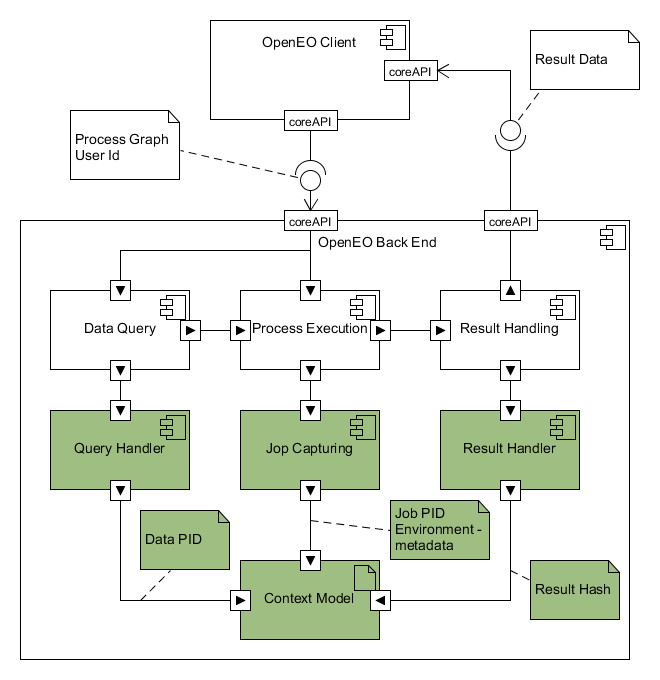
\includegraphics[width=\textwidth]{design_overview}
	\caption{Design Overview of capturing the job context model in bench marking mode.}
	\label{fig:design_overview} % \label has to be placed AFTER \caption (or \subcaption) to produce correct cross-references.
\end{figure}
That is how the benchmarking context model gets introduced. The idea is that not only the input data the whole process and the output data gets captured, but also every data in between of every process in the process graph. So for every process in the process graph the input, output data gets captured and the code executing the process. This makes it easier for users to see were the execution actually changed. But it also comes with higher implementation costs at the back end side. It also will affect the performance of the execution more than the common context model. The possibility of the implementation of such a granularity is also highly dependent on the back end implementation. Not every back end might be able to implement this into the back end due to execution optimization where the execution and results of the single  processes in the process graph are not distinctable. Nevertheless in theory the granularity does not have to stop there, the data and code could be captured for every line in the code. This flexibility of capturing makes it also a context model that  can be adapted to different use cases in the future.  

\subsection{User Interface}\label{Design:User Interface}

In this section the information for the users and how they are provided gets described. The capturing described in the previous sections consists of a lot of  information about the back ends that shall not be completely passed to the users in detail. For example it can be a security risk to provide specific programming language packages. On the other hand the users need to be able to see the differences of job executions and get environment information about the backends. Therefore there has to be a filter on which data can be shown to the user and what not. Every captured information is also not necessary interesting for the users. Data that is not secure to the user has to be defined by the different back ends themselves. The OpenEO project has a very diverse set of back ends and every one has a unique company security guideline. The important thing is that all of the information has to be captured and taken into account for the comparisons and they have to be open to the user.
Provenance information has to be provided to the user. Therefore there have to be new additions to to the core api specification. Additional endpoints for the users to get information about the back end has to be created in the Core API, back end and client. The following points summarize the the set of needed additions. 

\textbf{U1: Back end version}
There has to be an endpoint for users to retrieve back end specific information. The aim of it is to present the users with information about the current state of the back end and to help OpenEO users to decide which back end they want to use. There is already an endpoint defined in the OpenEO core API specification for the capabilities of the back end, where the back end information can be added. This addition to the API has of course to be implemented by every back end and client.

\textbf{U2: Detailed Job Information}
There is already an endpoint to get detailed information about the job status. But the provenance of the job is not in there yet, so it has to be specified in the API what information of the context model has to be provided there. At least the identifier of the input data and the identifier of the execution code has to be provided including the output hash for comparison.   

\textbf{U3: Comparing two Jobs}
The API has to add an end point for making it possible to compare two different jobs. There does not exist an endpoint for this in the 0.0.2 core API specification. The response of the comparison request needs to consist of what are the differences between two jobs. 


\section{Overview of Changes}\label{Design:Overview of Changes}
In this section the changes described in this chapter get summarized and assigned to the parts of OpenEO responsible for the tasks.
\todo{Make lists in the sections for better readability}
\subsection{OpenEO back end}\label{Design:OpenEO back end}
The openeo back ends need to implement the job dependent capturing as described in the section \ref{Design:Job dependent provenance} and implemented in section \ref{Implementation:Job dependent provenance}. The job dependent capturing is recommended to be implemented in the same programming language as the back end provider uses. The advantage of this is that the usage of the programming language is maintained anyway by the back ends to preserve the functionality of the processes and if the back end switches to a different location the setup of the capturing tool needs no further effort. 
The back end also need to run the job independent capturing described in section \ref{Design:Back end provenance}. This has to be run in a cron job or other automation tools so that the changes get notices by the tool. In section \ref{Implementation:Back end provenance} there is also an implemented tool doing so. 
In addition the backends need to implement the endpoints changes and additions of the OpenEO core API described in the next section.
\todo{add data identification changes}
\subsection{OpenEO core API}\label{Design:OpenEO core API}
The core API needs to add the endpoint for the version retrieval (e.g. at /version) end point. It is also possible to extend an existing endpoint for this purpose. 
There needs also an additional endpoint for comparing two different jobs. 
The process graph shall be extended by a timestamp to the product element so that it is possible to access deprecated data on the back ends.
\subsection{OpenEO Client}\label{Design:OpenEO Client}
The OpenEO clients need to implement the changes described above in the core API additions. In the OpenEO client the additional retrieved data needs to be visualized for a better user understanding.

\todo{maybe add overview picture}

\chapter{Implementation}\label{Implementation}
In this chapter the prototype of the concept described in \ref{Design} gets presented. The implementation consists of all suggested changes that need to be made to the OpenEO workflow including parts of the back end, core API and the clients. Thus all three parts of the OpenEO project architecture get modified in the implementation. There are several different back ends and clients implemented in parallel, which are all compatible with each other. One client and one of the back ends is used for the proof of concept of this thesis. The python client\footnote{https://github.com/Open-EO/openeo-python-client} is modified for the purpose of this thesis and for the back end the EODC back end\footnote{https://github.com/Open-EO/openeo-openshift-driver} gets used. Since python is the most used programming styles at the contributing back ends of the OpenEO project these implementations get used, because both of the chosen implementations are using python as the main programming language. So the adaptations described in \ref{Design} are implemented for the usage of the python client with the EODC back end. Both of the implementations are open source and can therefore be used by other backend providers with a similar setup.  

The implementation can be divided in four independent parts. In the following four sections these parts are described in detail. First the data identification implementation gets described, so the implementation of the RDA recommendations on the EODC back end. The next section is about the implementation of the automated back end provenance creation tool defined in section \ref{Design:Back end provenance}. After that there is a section about the job execution provenance as defined in \ref{Design:Job dependent provenance}. The last section is about the implementation of user interface additions defined in \ref{Design:User Interface}.     

\section{Data Identification}\label{Implementation:Data Identification}
\todo{Add info from EODC here and make a “how it was” and “how it will be/is now”}

\section{Back end provenance}\label{Implementation:Back end provenance}
The aim of the automated back end provenance computation is to make an easy to implement approach to capture all changes of the back end that have an influence on the back end processing results. In addition to this the implementation generates a back end version automatically on changes at the back end. The proposed tool can be used by every OpenEO back end with a Linux system. It is completely independent of the existing back end services, so it is an additional tool that has to be executed at the back end. In this section the implemented tool is called “BackendMonit”. 

\begin{figure}[h]
	\centering
	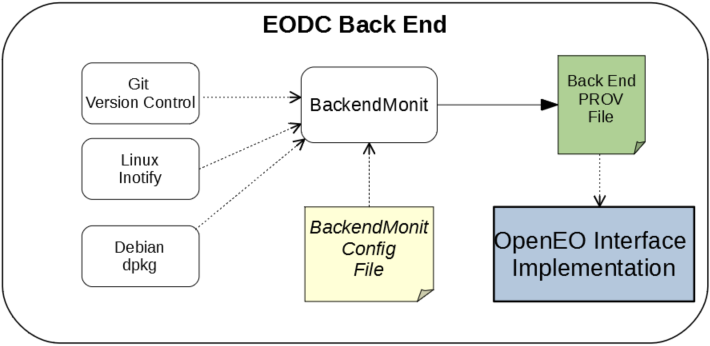
\includegraphics[width=\textwidth]{backendprov}
	\caption{Overview of BackendMonit inside of the EODC back end}
	\label{fig:backendprov} % \label has to be placed AFTER \caption (or \subcaption) to produce correct cross-references.
\end{figure}

BackendMonit is a stand alone capturing tool that gets called periodically as a cron job (see \cite{crontab}) by the back end hosting machine. EODC uses python as their default programming language on a Debian Linux based system, therefore the capturing tool is written in python and uses linux and debian tools. It is implemented in a way that other linux based back ends can use it to capture back end changes too, with some minor changes. The back end provenance tool uses a command line interface (CLI)  and a configuration file as a parameter. 
The workflow of running BackendMonit is as follows: 

\begin{enumerate}
	\item \textbf{Install Requirements} \\
	BackendMonit requires for the execution a view linux packages. First the tool runs on Python 3.6 hence it has to be installed on the system. There are no additional python packages necessary for it. Another requirement is inotify and dpkg, or any other packet management system for a Linux distribution. The version control system Git is also a requirement on the back end, since every back end has its own GitHub repository it is most probably already installed. 
	
	\item \textbf{Setup Configuration File} \\
	To make BackendMonit adaptable for other systems there needs to be a configuration file to configure the behaviour of it. The tool comes with a default configuration file, which the back end provider has to adapt to the back end. All paths to the tools described in the previous point is in the config file specified. Additionally, the path to the GitHub Repository used for the local back end repository is set in the configuration file and a list of folders, which are used by the back end provider for the execution of jobs, excluding temporary folders.      
	     
	\item\textbf{Starting Service} \\
	After the configuration is done, BackendMonit is executed in daemon mode, where it starts all processes of inotify to run in the background. To start the tool in daemon mode the "--init" parameter has to be set on execution. 
	
	\item \textbf{Start Cronjob} \\
	Now that inotify is configured and started as a service, BackendMonit has to check periodically if something changed on back end side. Therefore, the tool needs to be started every minute adding the "--check" parameter. Every time that happens it compares the current state of the back end with the current context model and if it differs it adds a new back end version with all metadata to the context model JSON file. 	 
\end{enumerate}

\textbf{Provenance Repository} \\
The context model of the back end provenance is a single JSON file that consists of all versions of the back end and their meta-data described below. In figure \ref{fig:backendprovcm} there is an example snipped of the provenance repository. 

\begin{figure}[h]
	\centering
	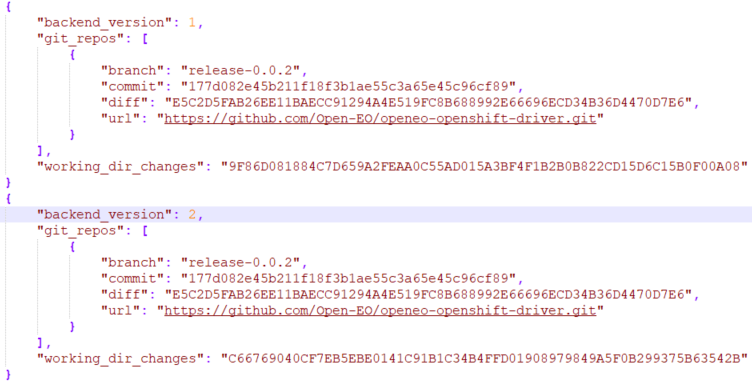
\includegraphics[width=\textwidth]{backendprovcm}
	\caption{Example snipped of the provenance repository of the EODC back end.}
	\label{fig:backendprovcm} % \label has to be placed AFTER \caption (or \subcaption) to produce correct cross-references.
\end{figure}

In the following it is explained how the in section \ref{Design:Back end provenance} defined provenance data points are read from the system by BackendMonit.  

\textbf{B1: Github Repository} \\
To capture the github repository, all folders that consists of github repositories have to be added to the configuration file. Git shall be installed at the back end and the path to the Git command has to be added to the configuration file as well. The monitoring tool will add the GitHub URL, the branch, the commit and a hash of all local differences to the context model. If there are any changes to the previous model there will be a new back end version.  

\textbf{B2: Used Folders} \\
Used folders by the back end have to be specified in the configuration file, excluding temporary folders and files. The tool daemon will check these folders on changes and will update the context model if anything changed at this folders. The tool used for this is inotify (see \cite{inotify}), this tool can be used to call a command if any changes on the file system in specific folders occur. The changes can be further specified by 12 different operations on the filesystem like IN\_DELETE, IN\_ACCESS. For the purpose of capturing changes to the used folder only write access on the folders trigger inotify.

\begin{lstlisting}[frame=single]
inotifywait -d -e modify -e attrib -e moved_to -e create -e delete DIR 
			-o outfile.log
\end{lstlisting}

\textbf{B3: OS and packages} \\
The linux operating system the eodc back end runs on is a debian based\cite{debian} operating system therefore the operating system release information and the packages can be retrieved with the debian packaging system (dpkg \cite{dpkg}).

\begin{lstlisting}[frame=single]
dpkg --get-selections
\end{lstlisting}

\textbf{B4: Core API Version} \\
The core API version will be added updated manually from the back end developers. Therefore the core API version is also read from the back end “GET /version” endpoint of the back end that returns the currently supported core API version. 

\textbf{B5: Back End Version} \\
The back end version begins with 1 and gets incremented on every change of the above described data. On every call of the cron job BackendMonit capture all above points and compares them to the most recent context model. If there are differences the version gets incremented by one and persisted in the context model. 


\section{Job dependent provenance}\label{Implementation:Job dependent provenance}
The capturing of the job dependent data is limited to the job execution modules of the EODC back end. The EODC back end of the release version "0.0.2" transforms the process graph into separate docker containers. For every process in the process graph there is a docker container created that runs python code with the input of the previous process. The first process docker container has the input data as input value. The result gets into a temporary folder separated by the different process result. Every process has its own temporary output directory until the whole process graph got executed, after that the temporary folders get deleted and only the result is saved and persisted.
To achieve the job provenance data capturing described in chapter \ref{Design:Job dependent provenance} the processes have to provide information about the input, output data and the processing itself. Two different implementations were created to achieve the job dependent provenance capturing. The first implementation uses the python code wrapper noworkflow \cite{c9e0604becba42af96a9cb0a6f60018b}. So instead of calling the processing with python, it gets called with the noworkflow wrapper that automatically creates a meta-data database about the python execution. The second implementation adds the specific information of interest to the logging of the processing and reads the logging files to generate the context model. The second implementation is in plain python. As described in the chapter \ref{Design:Back end provenance} the programming language of the back end shall be used for the implementation of the capturing tool. So the solutions use python to retrieve the needed provenance data. Both implementations have the same functionality and cover the full implementation of the described data of the Design section. 

\subsection{Provenance Repository}\label{Implementation:Provenance Repository}
There is a context model for each executed job, if the job gets re-executed, the context model gets replaced by the new context model. The job re-execution is internally handled as a new job with the same process graph. The functionality of letting the same job be re-executed without creating a new job id got dropped from the agenda of the OpenEO project in version 0.0.2 \cite{openeo}. 
The context model get persisted as a JSON file in the job execution directory. After the job carried out in the EODC back end the results are saved in a folder named after the unique job identifier. There the context model JSON file gets created by the implementations described below. The JSON file has the following structure:

\begin{figure}[h]
	\centering
	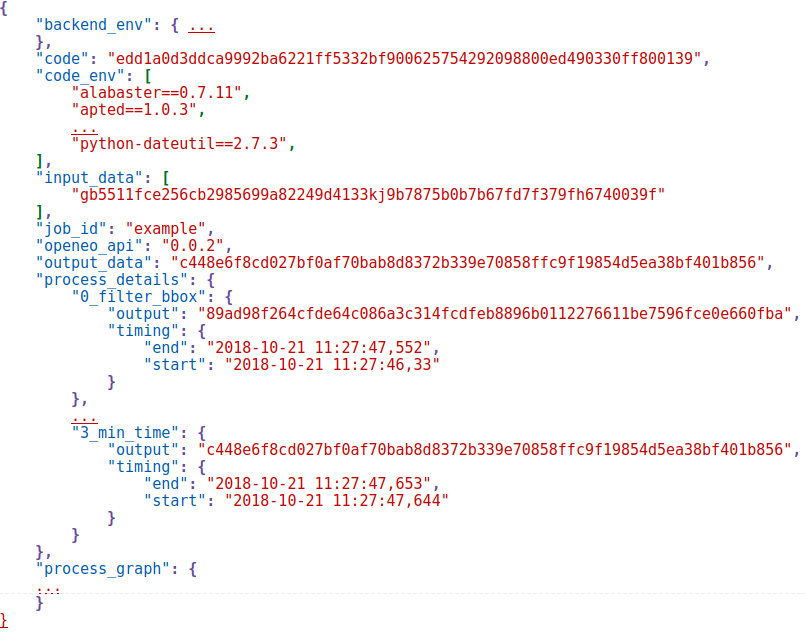
\includegraphics[width=\textwidth]{job_context_model}
	\caption{Design Overview of capturing the job context model.}
	\label{fig:job_context_model} % \label has to be placed AFTER \caption (or \subcaption) to produce correct cross-references.
\end{figure}
\todo{Update figure \ref{fig:job_context_model} input\_data identifier to the query store PID}

In figure \ref{fig:job_context_model} there is an example context model of a job execution. It consists of all points described for the context model in the Design section. In the following table there is the mapping between the context model definition defined in section \ref{Design} and key of the JSON context model file. 

\begin{table}[]
	\begin{tabular}{l|l}
		\textbf{Context Model Definition} & \textbf{JSON Key} \\ \hline
		\textbf{J1:  Source Input Data Identifier} & input\_data, process\_details \\ \hline
		\textbf{J2: Process Code Identifier} & code \\ \hline
		\textbf{J3: Programming Language} & code\_env \\ \hline
		\textbf{J4: Installed packages of programming language} & code\_env \\ \hline
		\textbf{J5: Start and End time of process execution} & process\_details \\ \hline
		\textbf{J6: Result Hash} & process\_details, output\_data \\ \hline
		\textbf{J7: Back end provenance} & backend\_env \\ 
	\end{tabular}
\end{table}

The mapping described in the table above is implemented by both solution systems. 

\subsection{Benchmarking Mode}\label{Implementation:Benchmarking Mode}
As defined in section \ref{Design:Job dependent provenance} there is also the optional possibility to capture not only the overall process, but also every process and the data in between for comparison reasons. 
If the process executed is not the first one and the benchmarking capturing mode is on, the input data identifier gets replaced by the output hash of the previous process. The scope of the benchmarking is just to make it able to see differences in the executions, but not to be able to identify the differences. Hence, a hash of the previous output data is sufficient. The hash gets created after the execution, by creating the hash of the execution at temporary output directory of the previous process. The EODC back end creates for each process execution a temporary folder where the output data of every process is stored, after the execution the temporary folder gets deleted. Between the finished execution and the deletion of the temporary folders a self provided python function gets called to make an SHA-256 hash over the results. In the benchmarking mode not only the data gets captured between the processes but also the timing of the single process executions. This is done by adding logging messages for the start and end of the process execution. The logging file is afterwards parsed and the timestamps are copied to the context model. Last but not least the identifier of the code is captured, by reading the git information out of the back end provenance. For the user convenience the url of the process code on GitHub with the currently checked out commit is added to the context model. Both implementations have the benchmarking realized as described before.    
%\todo{Implement an switch to make it optional with the time stamps of the processing}

\begin{figure}[h]
	\centering
	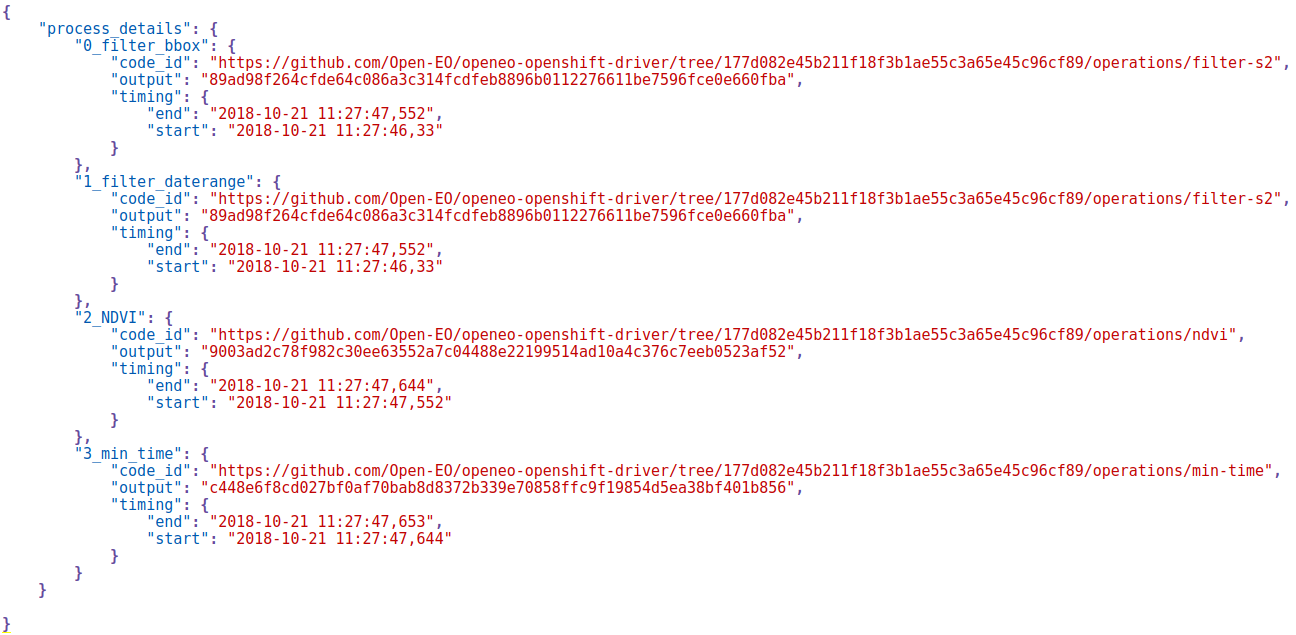
\includegraphics[width=\textwidth]{benchmarking_pg}
	\caption{Example of an benchmarking mode snipped out of the process graph.}
	\label{fig:benchmarking_pg} % \label has to be placed AFTER \caption (or \subcaption) to produce correct cross-references.
\end{figure}

In the following two sections the process of capturing the context model in two different implementation approaches get explained further. First the approach of using noworkflow as capturing tool and second the implementation with plain python and logging. 

\subsection{Noworkflow Implementation}\label{Implementation:Noworkflow Implementation}
Noworkflow is a python module used to capture the provenance of a python script execution. The main aim of it is that the program itself does not have to be changed, it only has to be executed with the noworkflow interpreter instead of python. It then automatically creates a provenance database on every execution of the script called “trial”. Every execution creates a new trial. A trail in the past can be re-executed with the same conditions and the trails itself can be easily compared and visualized with noworkflow \cite{c9e0604becba42af96a9cb0a6f60018b}. Noworkflow and its capabilities are described in section \ref{Noworkflow}. 
For the purpose of the job dependent provenance capturing described in the Design section, only parts of the provenance capturing functionality that noworkflow offers gets used.    

\begin{figure}[h]
	\centering
	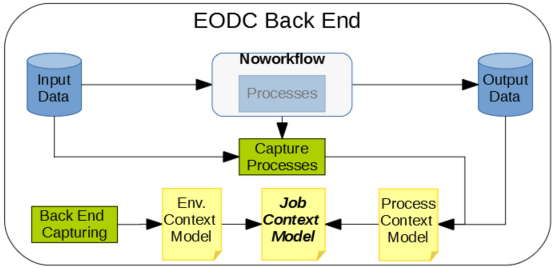
\includegraphics[width=\textwidth]{noworkflow_impl}
	\caption{Overview of the noworkflow implementation.}
	\label{fig:noworkflow_impl} % \label has to be placed AFTER \caption (or \subcaption) to produce correct cross-references.
\end{figure}

\textbf{J1:  Source Input Data Identifier} \\
The source input data identifier is the id for the input data and query provided by the EODC query store described in section \ref{Implementation:Data Identification}. 


\textbf{J2: Process Code Identifier} \\
The job identifier is defined by the back end version, which includes the current state of the locally checked out GitHub repository.\\
To make a more detailed comparison possible there gets also the hash of the executed code added to the context model.The job execution runs with noworkflow and for every execution there is a noworkflow trial created that consists of the hash of the executed code. The hash from the database of noworkflow gets retrieved via the command line interface. It contains the command “show” (see code block below), which returns the data of a specific trial. The code hash gets extracted from the output and added to the context model for easy comparison reasons. 

\begin{lstlisting}[frame=single]
now show --dir=JOB_DIR
\end{lstlisting}

\textbf{J3 and J4: Programming Language and  Installed packages of programming language} \\
The programming language gets captured with the modules of the python packages in the noworkflow database. To retrieve the modules the command line interface is used with the command “-m” (see code block below) that returns all used python modules including the version of python used to execute the code. In the context model the python version is in the list of used python tools returned by the noworkflow command. The data is restructured to fit in the JSON output file and represented by a list. 
%\todo{Add programming language to code capturing + noworkflow version see pkg\_resources and sys.version\_info[0]}

\begin{lstlisting}[frame=single]
now show -m --dir=JOB_DIR
\end{lstlisting}

\textbf{J5: Start and End time of process execution} \\
The start and end time of the processes gets captured through the logging of the processes. Every process writes to a logging file the start and end time of the execution. The data is human readable to provide the user retrieving the context model more comfort. The used format is “yyyy-MM-dd hh:mm:ss”. The seconds have three digits for more precise time stamps. All log files are in the job execution folder, where the data gets persisted. After the execution when the context model gets created the timestamps are read from the log file and added to the context model of the processes.  

\textbf{J6: Result Identifier} \\
The result identifier consists in the common capturing mode of the output data of the whole process graph execution. It is a SHA-256 hash of the resulting sorted output files, which are placed in the results folder of the job execution directory. The order id is a counter that starts with zero and increments for each process executed. It describes in which order the processes get executed. It is used in the context model to get feedback about the execution order of the processes.

\textbf{J7: Back end provenance} \\
The back end provenance is read from the BackendMonit context model JSON file at the back end described in section \ref{Implementation:Back end provenance}. Provenance of the latest back end version gets copied to the context model. The whole back end provenance get included to the context model so that the environment is independent of the persistence of the back end provenance file. 

\subsection{Python Implementation}\label{Implementation:Python Implementation}
The noworkflow tool needs some additional requirements to the back end provider and slows down the processing, because the granularity of the code capturing is much higher than needed. These are the reasons why back end provider might not want to use the provenance tool in a productive server. The EODC implementation proposed by this thesis is an example for other back ends and hence needs to be easy to implement. So another solution for capturing the processing is implemented in pure python. 
The python solution uses logging messages to transfer the needed data from the process execution program to the capturing tool that reads the logs after the job is finished. This needs no additional python packages and the execution can stay the same. The only changes to the original server implementation is the new logging messages that have to be added to the already existing logging framework at the EODC back end. An overview of the logging and capturing process of this solution can be viewed at figure \ref{fig:python_impl}. 

\begin{figure}[h]
	\centering
	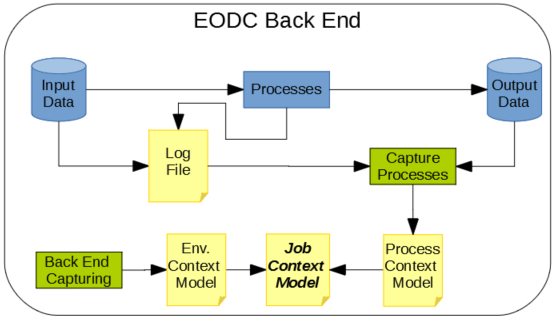
\includegraphics[width=\textwidth]{python_impl}
	\caption{Overview of the python implementation.}
	\label{fig:python_impl} % \label has to be placed AFTER \caption (or \subcaption) to produce correct cross-references.
\end{figure}

\textbf{J1:  Source Input Data Identifier} \\
The source input data identifier is the id for the input data and query provided by the EODC query store described in section \ref{Implementation:Data Identification}. 

\textbf{J2: Process Code Identifier} \\
The job identifier is defined by the back end version, which includes the current state of the locally checked out GitHub repository.\\
To make a more detailed comparison possible there gets also the hash of the executed code added to the context model. In the python solution a SHA-256 hash gets generated over the whole source code used for the job processing. 

\textbf{J3 and J4: Programming Language and  Installed packages of programming language} \\
The programming language of the EODC back end is python and also the capturing tool is written in python. To list all installed packages in python “pip” can be used. With the python module “pip” the installed python modules can be managed. The EODC back end GitHub repository has a python environment file to automatically install all needed dependencies of python via “pip”. A feature of that tool is the “pip freeze” call, which returns all installed python packages including their versions. This gets translated to a JSON list object and saved to the context model. In addition to this the python version gets captured by the "sys.version" call of the python capturing tool.    
%\todo{Add programming language to code capturing see sys.version\_info[0]}

\textbf{J5: Start and End time of process execution} \\
The start and end time capturing is the same as described in the noworkflow implementation see section \ref{Implementation:Noworkflow Implementation}.

\textbf{J6: Result Identifier } \\
The result identifier is implemented in the same way as the noworkflow implementation see section \ref{Implementation:Noworkflow Implementation}

\textbf{J7: Back end provenance} \\
The back end provenance information is implemented in the same way as the noworkflow implementation see section \ref{Implementation:Noworkflow Implementation}

\section{User Interface}\label{Implementation:User Interface}
The user interface implementation is done by adding endpoints to the existing OpenEO core API version 0.0.2 and applying the additional endpoints to the python client and the EODC back end. The relevant additions defined in section \ref{Design:User Interface} are implemented in the following way:

\textbf{U1: Back end version} \\
Retrieving additional information about the back end was added into a new defined end point of the API. The new endpoint is a GET request called “/version”. The user does not have to be logged in to access this endpoint. Response of the version endpoint is in the implementation the whole job independent provenance information of the back end, like defined in section \ref{Implementation:Back end provenance}. In a productive version the data may be filtered for information marked as a security risk. This endpoint was added to the EODC back end and to the python client so that the user can call a method in the python client called “version()” to retrieve the information of the back end directly in the python environment. 
\todo{explain in detail what info was included here and how it got captured}

\textbf{U2: Detailed Job Information} \\
There is already an endpoint to get detailed information about the job status. It is the existing “GET /jobs/<job\_id>” endpoint of the core API, which by the version of 0.0.2 only contains the execution state of the job and the job id. In addition to the already available information the whole job dependent provenance gets added to this endpoint in the implementation of this thesis. The python client got also changed to match the end point changes described before.  
\todo{explain in detail what info was included here and how it got captured}

\textbf{U3: Comparing two Jobs} \\
The comparison of two jobs is not defined in the version 0.0.2 of the core API, hence there does not exist any. So a new one has to be defined in a manner of the existing endpoint definitions. For the purpose of this thesis the endpoint  “POST /jobs/<job\_id>/diff” gets introduced. In the url of the request you define the base job id that has to be compared with other jobs. In the body of the request the job ids that the base job shall be compared with are defined in a JSON list. After getting the request from the user, the back end compares the context models of the base job with every job in the request body list. The result consists of for every item in the base job context model the term “EQUAL”, if the item is the same in both jobs, “DIFF”, if the items are not the same in both jobs, or “MISSING”, if the item is in the base job, but not in the target job of the request list. This can occur if the context model was modified in the future and some additional fields of it are not in the context models of the past or in the benchmarking mode if one process graph has mode processes defined than another one. The response consists of the context model of all jobs with one of the previously described three states inside of every items value. In the python client this feature was added and in addition there got an visualisation implemented to make the differences of the context models more visible to the users.

\todo{Maybe also add image of REST request \& response.}
\todo{Add image of the client visualisation}

In addition to the implementations defined before, a translation tool for the context model got implemented. It transforms the job dependent context model into a PROV-O specified file. This is only realized in the benchmarking mode of the back end and it describes the job execution steps. The mapping of the context model to the PROV-O standard is as follows.

\todo{describe PROV-O  export of Context Model}
\todo{add image of the PROV-O export} 

\section{Implementation Overview}\label{Implementation Overview}

\subsection{Changes to Client}
\subsection{Changes to Core API}
\subsection{Changes to Back end}
\todo{Add the big picture of all components and their additions}

\chapter{Evaluation}\label{Evaluation}
In this chapter the implementation gets tested and evaluated. By running the use cases it gets evaluated if the implementation reaches the aim of the thesis. First the RDA data identification recommendations are checked with the implementation and how they apply or not need to apply. Then the two implementations are compared with each other. The last section in this chapter is testing the in section \ref{Use Cases} defined use cases against the implementation. 

\section{Data Identification}\label{Evaluation:Data Identification}

\begin{itemize}
	\item \textbf{R1: Data Versioning}
	\item \textbf{R2: Timestamping}
	\item \textbf{R3: Query Store Facilities}
	\item \textbf{R4: Query Uniqueness}
	\item \textbf{R5: Stable Sorting}
	\item \textbf{R6: Result Set Verification}
	\item \textbf{R7: Query Timestamping}
	\item \textbf{R8: Query PID}
	\item \textbf{R9: Store the Query}
	\item \textbf{R10: Automated Citation Texts}
	\item \textbf{R11: Landing Page}
	\item \textbf{R12: Machine Actionability}
	\item \textbf{R13: Technology Migration}
	\item \textbf{R14: Migration Verification}
\end{itemize}

\todo{Compare implementation with the recommendations. So how it was and how it is.}

\section{NoWorkflow vs Python Implementation}\label{Evaluation:NvsP}
The two implementation approaches are implementing the same features, even though there are major differences between them. In this sections the different implementations get compared and the advantages and disadvantages of them get discussed. Therefore three categories get confronted by both implementations. First the effort of applying the implementation gets compared, then the performance of the python and the noworkflow implementation is compared. The last comparison is about the maintenance and the extensibility of the solutions. 

\subsection{Implementation Effort}\label{NvsP:Implementation Effort}
The implementation of this thesis applies the purposed reproducibility context model creation only for the EODC back end. There are six other back end providers in the project were there needs to be a solution too. Therefore the effort of the implementation gets graded so that other back end providers can decide, which solution they want to implement.

\textbf{noWorkflow} \\
The implementation of noworkflow is by the definition of noworkflow itself quiet easy. The EODC back end is a python implemented back end and therefore just the call of the python scripts has to be changed to the noworkflow command line interface, which is a wrapper around python. That was everything that has to be done on the code provenance capturing part. The created database has to be moved to the job output folder. To get the provenance data the command line tool has to be called, so there is some effort to find the needed data in the documentation of the tool. After finding the information it has to get parsed for the information needed for the context model, which takes some effort, but can be done in a view hours. 

\textbf{Python} \\
The python implementation does not affect the processing code of the EODC back end, but adds some additional logging calls to it. So that the actual code has to be modified, which takes longer than the noworkflow implementation. After the logging calls are added to the code the capturing part is done. For retrieving the information of the logging file it has to get parsed to transfer it to the context model of the job. This is easily done, because the added logging messages are only the needed information and it is self formatted so that the parsing is easy to implement.   

\textbf{noWorkflow vs Python} \\
The implementation effort of both solutions are very similar, the noworkflow solution has the advantage, that the capturing does not require changes in the code. The downside of noworkflow is that it captures much more provenance information than needed for the context model and the needed information has to be extracted from the database in case to get it. 

\subsection{Performance}\label{NvsP:Performance}
Most of the OpenEO back end provider have customers that pay by the length of the execution time and therefore the provenance capturing addition has to affect performance as little as possible. Therefore the performance of the two implementations get compared.

\textbf{noWorkflow} \\
Due to the wrapper around the python interpreter, the performance after applying the solution was very low. The execution time a bit more than three times the original execution without capturing. The fact about the bad performance of noworkflow is the reason for the implementation of the python solution. 

\textbf{Python} \\
The python implementation adds almost no overhead to the execution. The parsing of the log file is the only part of the python code that has an real effect on the performance. Hence, the execution duration using the python solution is only a view milliseconds longer compared to the unmodified execution.  

\textbf{noWorkflow vs Python} \\
The python implementation is by far much more efficient when it comes to performance. The main reason is the wrapper around python and the high amount of captured data in the noworkflow solution of data that is not needed in the context of this thesis. In the table below the timings of the proof of concept execution is recorded. The timing in the table is the time between sending the request and getting response from the server about the finished processing. 

\begin{table}[]
\centering
	\begin{tabular}{l|l|l}
		\textbf{original execution} & \textbf{noworkflow solution} & \textbf{python solution} \\ \hline
		4069 ms & 11900 ms & 4074 ms \\ 
	\end{tabular}
\end{table}

\subsection{Maintenance and Extensibility}\label{NvsP:Maintenance and Extensibility}
OpenEO is still involving and will be in the future due to the rapidly changing earth observation market. So in this section the extensibility and the maintenance of the solutions gets compared. 

\textbf{noWorkflow} \\
NoWorkflow is already capturing much more information about the execution. It also comes with a high amount of features to query the provenance data and to visualize it. NoWorkflow is also still evolving and new features may be added to it in the future. On the other hand the noworkflow solution is depending on the external maintenance of noworkflow, which is not guaranteed. So it can happen, that noworkflow does not work with a new python version, or if the back end provider switches to another programming language noworkflow can not be used any more. In addition to this disadvantages it is hard to add additional provenance data that is not already captured by noworkflow, because then noworkflow has to be adapted.

\textbf{Python} \\
The python solution is only capturing exactly the information that the back end provider wants it to capture. On fine granulated capturing and parsing the additional effort can be quite high. The advantage on this implementation is that the tool is easy extensible by just adding more logging information. Since logging is a simple feature of python it can be assumed that it will not change much in the future. If the back end provider decides to switch to a different programming language it can easily switch by adapting the code parsing to the new language and add the logging messages to the new back end implementation. 

\textbf{noWorkflow vs Python} \\
Noworkflow comes with more features, especially for the back end provider to query and visualize the provenance data, but it is much harder to add information to the provenance capturing mechanism. So the python solution is much more flexible on changes and more independent from the environment than the noworkflow implementation.  

\section{Use Cases}\label{Evaluation:Use Cases}
In this section the use cases introduced in section \ref{Use Cases} are tested against the python implementation. The setup of the evaluation is on the back end side the EODC python implementation described in section \ref{Implementation:Python Implementation}. To communicate with the back end the modified python client gets used. The modifications to the python client are described in \ref{Implementation:User Interface}. The use cases get evaluated by trying to apply them on the original OpenEO setup (version 0.0.2) and comparing it to the implemented additions described in section \ref{Implementation}. The release-0.0.2 OpenEO set up is named original set up for convenience reasons and the OpenEO set up with all, in this thesis described, changes is called modified set up. An Overview of the evaluation is visualized in figure \ref{fig:usecases_eva} 

%\begin{figure}[h]
%	\centering
%	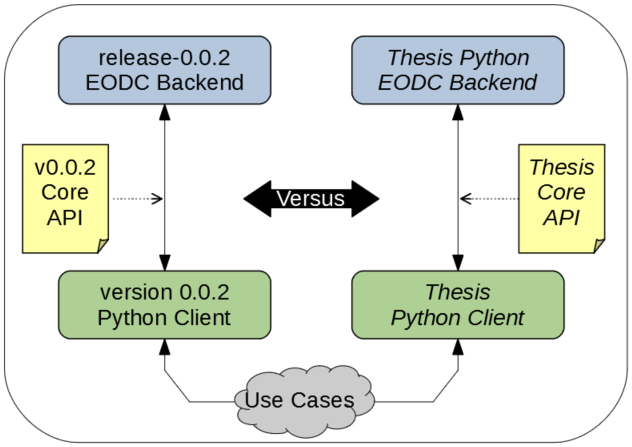
\includegraphics[width=\textwidth]{usecases_eva}
%	\caption{Overview of the evaluation setup }
%	\label{fig:usecases_eva} % \label has to be placed AFTER \caption (or \subcaption) to produce correct cross-references.
%\end{figure}

\subsection{Capturing the Back-end environment}\label{Evaluation:Use Case1}
The first Use Case can be seen from two perspectives. From the back end providers point of view and from the users point of view. The user wants to get information about the back ends provenance and the current version. The back end provider wants to have an automated tool to capture the provenance data and to create automatically back end versions. This is done in the implementation by running the BackendMonit tool described in section \ref{Implementation:Back end provenance}. The back end provider has just to start the service of BackendMonit and the capturing and back end version creation will be done automatically. 
Users will use an OpenEO client to access the back end. Therefore, in the following the use case gets visualized by the view of an OpenEO user using the python client: 

\textbf{Original Setup}

\textbf{Modified Setup}


\todo{Run Test case 1 and show how it was and how it is now.  + Python Client Results}

\subsection{Capturing job dependent environments}\label{Evaluation:Use Case2}
\todo{Run Test case 2 and show how it was and how it is now.  + Python Client Results}

\textbf{Original Setup}

\textbf{Modified Setup}

\subsection{Getting differences of job executions}\label{Evaluation:Use Case3}
\todo{Run Test case 3 and show how it was and how it is now.  + Python Client Results}

\textbf{Original Setup}

\textbf{Modified Setup}

\chapter{Conclusion and future Work}\label{Conclusion}

\section{Conclusion}

5.	Summary of thesis
6.	Describe limitations
7.	Describe noworkflow and python implementation differences 
8.	Describe possibilities
9.	Describe improvements

\section{Future Work}
In this thesis a concept for applying reproducibility in the OpenEO project is purposed. Still there are major issues to be addressed in the future of the OpenEO project. There are several ways to improve the concept and many open questions, which are open for the future. \\
OpenEO is still evolving until the project end 2021 and also afterwards. There are a lot of features that have to be defined and may interfere with the concept proposed in this thesis. User defined functions are part of the project and to be capable of reproduce them can lead to adaptations to the concept. Another main issue of the OpenEO project is the billing concept that has to be apply-able to a diverse set of back ends. Since the capturing process and the generation of the context model takes time it has to be considered in the billing plan of the back ends. The growing diversity of the back ends applying the OpenEO standard is a huge challenge to the design of the context model of this thesis.\\
The storage of the context models in JSON files was used in this thesis , but has definitely limitations that have to be addressed in the future e.g. the querying over the data sets. 
In the solution of this work the data is captured for identifying how jobs are executed and to be able to identify how the job was executed. An addition to this can be a way to automatically apply the reproduction of an executed jobs of the past. To achieve this a method of validating the output of a job execution needs to be introduced. The possibility to get automated data and process citation to researchers of OpenEO interfaces is also a possible future work. Special users may need a finer granularity of the process capturing, leading to a definition of scalability of the processing capturing.      


\backmatter

% Use an optional list of figures.
\listoffigures % Starred version, i.e., \listoffigures*, removes the toc entry.

% Use an optional list of tables.
\cleardoublepage % Start list of tables on the next empty right hand page.
\listoftables % Starred version, i.e., \listoftables*, removes the toc entry.

% Use an optional list of alogrithms.
%\listofalgorithms
%\addcontentsline{toc}{chapter}{List of Algorithms}

% Add an index.
\printindex

% Add a glossary.
\printglossaries

% Add a bibliography.
\bibliographystyle{alpha}
\bibliography{intro}

\end{document}